%!TEX encoding = UTF-8 Unicode
%!TEX program = xelatex

\documentclass[bachelor,english,numbers]{ustcthesis}
% bachelor|master|doctor [professional] [english] [pdf] [authoryear|numebers]

\usepackage{ustc-package}

\graphicspath{{figures/}} %%%%%%%%%%%%%%%%% directory of pictures

\title{具有赝磁场的石墨烯中的\\复合费米子液体理论}
\author{胡啸东}
\major{理论物理}
\supervisor{副教授\ 刘国柱}
\cosupervisor{副教授\ 吴英海}
% \date{二〇一七年五月一日}    % 注释掉则为今日
% \professionaltype{专业学位类型}
% \secrettext{机密\quad 小于等于20年}    % 内部|秘密|机密,注释本行则不保密

\entitle{Composite Fermion Liquid\\in Graphene with\\Pseudo-magnetic Field}
\enauthor{Xiaodong Hu}
\enmajor{Theoretical Physics}
\ensupervisor{Prof. Guo-Zhu Liu}
\encosupervisor{Prof. Ying-Hai Wu}
%\ensupervisor{Prof. Luogeng Hua}
%\encosupervisor{Prof. Xuesen Qian}
% \endate{May 1, 2017}    % today if commented
% \enprofessionaltype{Professional degree type}
% \ensecrettext{Confidential\quad Less than or equal to 20 years}
% Internal|Secret|Confidential

\begin{document}

\maketitle

% 本科论文:
%   frontmatter: 致谢、目录、中文摘要、英文摘要
%   mainmatter: 正文章节、参考文献
%   appendix: 附录
%
% 硕博论文:
%   frontmatter: 中文摘要、英文摘要、目录、符号说明
%   mainmatter: 正文、参考文献
%   appendix: 附录
%   backmatter: 致谢、发表论文

\frontmatter

\begin{acknowledgements}
	I chrished the final time in USTC and was fortunately being supervised by two teachers during my research on this problem. I appreciated the theoretical guidance of Prof. Guo-Zhu Liu in USTC, without whom I cannot get out of mire when recovering the tedious computation details of HLR's theory during my winter vacation. I benefit a lot from his guidance of functional path integral formalism, which accelarated my understanding of the relevant chapters of Altland\&Simons's book and calculation of the matrix element of polarization tensor. His course \emph{Quantum Many Body Physics} also endowed me a solid foundation on theoretical condensed matter physics. I also appreciated the physical instruction from Prof. Ying-Hai Wu in HUST. Weekly exchanges with him cleared all my vagueness about the physical picture of the $\mathcal{K}$-matrix with high degenerency and multi-layer flux attachment. These discussions also prevented me from the potential deviation from the mainline --- once I naively insisted that we should develop a Fermionic Chern-Simons theory for massless Dirac fermions, it was his distinct demonstration terminated my divergent thoughts and helped me re-focus on our project.\par
	
	Moreover, frequent academic exchanges with my best friend Zhihao Zhang galvanized a logic derivation to the singular gauge transformation and Chern-Simons action. In fact, apart from my dissertaion, whenever I look back my life in USTC, there was always a figure of him residing in my fragments of memory. I believe our intimate friendship and relation of mutual promotion will extend to the rest of life. Academic debates with my roommate Shu-xuan Wang also helped me clarify some sublte concepts. Frankly, the first time I observed the close relation of functional mean-field methods and spontaneous symmetry breaking happened in the dormitory. An anonymous answerer on Chinese Q\&A website \texttt{zhihu} also provided me with some information about half-filling FQHE at the frontier of research. So here I sincerely express my gratitudes to them as well.
\end{acknowledgements}

\tableofcontents

%\listoffigures
%\listoftables
%\listofalgorithms
%\input{chapters/notation}

\begin{abstract}
	我们在本文中发展了一套研究石墨烯中朗道填充因子 $\nu=1/2$ 且非极化填充的有效理论,计算了它在由扭曲石墨烯造成的反向赝磁场激励下的电磁响应与霍尔电导。\par

	在部分填充的情况下,由于费米子被限制在最低朗道能级,当我们将原来的万尼尔表象下的场算符变换到朗道能级波函数的表象上时,发现子格点简并度与谷简并度合二为一,故而根据本征函数的性质,可以用有质量的二次型色散关系的准粒子哈密顿量来有效地描述石墨烯中的无质量狄拉克费米子。而尽管表象变换后一般能级的库伦相互作用变得极为复杂,对于我们关注的最低朗道能级的情况,计算后依旧可以采用原来的相互作用形式。因此我们的哈密顿量与正常的半导体单分量分数量子霍尔效应的差异仅仅在于谷简并带来的多分量。\par

	基于非极化填充的多分量 Chern-Simon 理论,我们在反向赝磁场下计算了电磁响应张量。发现它的激发谱,无论是有能隙的分数量子霍尔态激发,还是无能隙的激发,都与正常半填充因子分数量子霍尔效应的结果一模一样;但是在我们的独特激励下,它的径向响应变为正常半填充因子情况的两倍,而静态横向电导精确等于零。通过表面声学波实验,可以验证石墨烯在分数填充因子下我们的非相对论费米型 Chern-Simons 理论的有效性。

	\keywords{石墨烯;赝磁场;分数量子霍尔效应;费米型 Chern-Simons 理论}
\end{abstract}

\begin{enabstract}
	We develop an effective theory of unpolarized states in half-filled graphene, studying the electromagnetic response and Hall conductance under the pseudo-magnetic field induced by symmetrical strain on graphene.\par

	In the case of partial filling, when we perform the representation transformation from Wannier function to Landau Level (LL) wave functions, one finds that the valley degenerency coincides with the sublattice degenerency at the lowest LL. So in terms of the form of eigen functions, we can make use of the Hamiltonian of massive particles with parabola dispersion relation to discribe the massless Dirac fermions in graphene. Although the expression of Coulomb interaction becomes extremely complicated after transforamtion of representation for general LL, in the situation what we concern with, where only the lowest LL is occupied, original form of interaction never becomes futile after computation. Thus the only difference of our theory to that of fraction quantum Hall effects (FQHE) in usual semiconductors comes from the more freedoms brought by the valley degenrency.\par

	Based on the fermionic Chern-Simons theory of unpolarized states, we calculate the electromagnetic response tensor under the stimulus of opposite pseudomagnetic field and find that the excitation spectrum, whatever gapped FQHE states or gapless one, concides with that of ususal partially filled FQHE. But our special stimulus makes the longitudinal reponse double and the static transverse conductance vanish. The effectiveness of our theory can be confirmed by the accurate surface acoustic wave experiments.  

	\enkeywords{Graphene; Pseudo-magnetic Field ; Fractional Quantum Hall Effect; Fermi-onic Chern-Simons Theory}
\end{enabstract}


\mainmatter

\chapter{Introduction}
	\section{Historical Review of Experimental Results}
		\indent\par The integer quantum hall effect (IQHE) was first observed in two-dimensional electron gas (2DEG) electrostatically induced by metallic gate valtage on Silicon MOSFET or by modulation dopped GaAs-AlGaAs heterostructure by von Klitzing \cite{klitzing1980new,von1986quantized,comtet2000aspects}. Stark contrast is observed on the stepwise dependence on strong magnetic field, as compared to a linear dependence as in classical Hall effect. Those step Hall resistances, or plateaus, quantized with extreme high resolution as $\frac{h}{ne^2}$ with an \emph{integer} $n$, while the corresponding longitudinal resistance drops sharply to zero in the meanwhile. The high resolution even made quantum Hall effect (QHE) as the resistance calibration standard since 1990.\par

		Two years after the first observation of IQHE, fractoinal quantum Hall effect (FQHE) was discovered by Tsui, Stormer and Gossard \cite{tsui1982two,stormer1999fractional} in a much lower temperature and higer magnetic fields enivronment on a higher mobility 2DEG of Si-dopped GaAs-AlGaAs heterojunctions. FQHE possesses an analogous characteristic as QHE, except that the quantized Hall resistance is $\frac{h}{e^2}$ divided by a \emph{fraction}. The first observed fraction is $\nu=1/3$ and about $100$ fractional quantum Hall states have been observed so far \cite{laughlin1983anomalous}. Most of these fractions are of odd denominator, but the existence of even denominator FQHE states like $\nu=1/2,5/2$ aroused huge theoretical interests in this field.\par
		%Other non FQH states, like marginal Fermi liquid state $1/4,1/2$ and stripe state , also arouse huge interests.
		
		Regarless how the 2DEG is formed, Berry phase and impurity-induced localization \cite{von1986quantized,tong2016lectures} are widely accepted as the cause of IQHE\footnote{TKNN theory \cite{tong2016lectures} also provide one explanation of IQHE.}, and interplay of kinetic energy and interaction results in FQHE \cite{simon1998chern}. So besides the familiar heterostructures like Si-MOSEFT or dopped GaAs-AlGaAs, Graphene and other two-dimensional materials are also believed to host IQHE and FQHE. And experimentalists did find a slightly distinct quantized Hall conductance in graphene \cite{zhang2005experimental} that $\sigma_{xy}=\pm4(n+\frac{1}{2})\frac{e^2}{h}$. The factor $4$ comes from the spin degenerency and valley degenerency of graphene, and the extra translation $\frac{1}{2}$ can be explained by Berry phase or relativistic Dirac equation \cite{sarma2011electronic}.\par

		FQHE in graphene was also found four year latter in a suspended graphene with high mobility comparable to some good quality 2DEG in GaAs-AlGaAs heterostructure in \cite{du2009fractional,dean2011multicomponent}. Both groups of Du {\it et al.} and Dean {\it el al.} merely found odd denominator fraction states. But in 2014, even denominator states are also observed in suspended graphene \cite{ki2014observation}. Therefore, motivated by rich physics hidden in even denominator FQHE in GaAs, it's valuable to study the electromagnetic tranports in graphene with even denominator Landau Level (LL) filling factors as well, particularly, we concentrate on the case of $\nu=1/2$ in this paper.

	\section{Composite Fermions and Chern-Simons Theory}
		\indent\par The concept of \emph{composite fermion} stem from the Jain's famous paper in 1989, in which a mapping between the wave functions of IQHE states and approximate --- but extremely good --- wavefunctions for FQHE states is keenly pointed out \cite{jain1989composite}. This wave function mapping can be regared as attaching an \emph{even} number of vortices of the wave function to each electron, turning it into a ``composite'' fermion.\par

		Although the idea of composite fermion suffered some resistance from the theoretical community at first, its validity was gradually accepted and the idea was further developed by many groups. S.C. Zhang {\it et al.} shot to fame with their model of bosonic Chern-Simons theory, in which \emph{odd} number of flux is attached and incompressible excitation of FQHE states are explained by the Ginzberg-Landau theory of symmetry breaking \cite{zhang1989effective}. Approaches of fractional statistics and Chern-Simons field also culminate the field of anyon superconductivity \cite{wilczek1990fractional,chen1989anyon} for a time.

		\subsection{Single-layer Fermion Chern-Simons Theory}
		\indent\par The fermionic Chern-Simons field theory proposed by Lopez and Fradkin in \cite{lopez1991fractional} comes to epitomize the development of field theory formalism on FQHE, providing a systematic (or at least semi-systematic) perturbation calculations of quantities such as longitudinal and transverse conductivities that are experimentally measurable. And formal study of the relation of wave function of ground state with the generating function of green function at equal time in \cite{fradkin1993wave} enable Fradkin to bridge the field theory formalism to Jain's trial series of incompressible FQHE wave functions. Shortly thereafter, the half-filling state is also well described by Halperin, Lee, and Read's famous work \cite{Halperin1995Theory} (known as HLR) with this approach, surprisingly indicating that unlike incompressible FQHE states with odd denominators, the even denominator states like $\nu=\frac{1}{2},\frac{1}{4}$ are rather compressible and Fermi-liquid-like\footnote{More precisely, the behavoir of \emph{infrared divergence} of the effective mass of composite fermions \cite{stern1995singularities} reveals that even denominator states are \emph{marginal Fermi liquid}. But theoretical framework of normal Fermi liquid aptly fit the physical picture of this system with just a slight but reasonable modification of the model.}.
		%Though effective enough on odd fraction quantized Hall conductance, S.C. Zhang's theory cannot interpret the whole hierachical structure of FQHE, neither can it  a field theoretical formalism was developed that roughly corresponded to Jain’s composite fermion wavefunction approach 13 – 15 . In these Chern-Simons approach, electrons is modeled as fermions bound to an even number of fictitious flux quanta which in some sense represent the even number of vortices of Jain’s composite fermion. The great advantage of this Chern-Simons approach is that it allows for simple yet systematic (or at least semi-systematic) calculations of quantities such as conductivities that are measurable experimentally.\par
	\subsection{Multi-layer Fermionic Chern-Simons Theory}
		\indent\par A richer variety of states will emerge if more freedoms is added in Fermionic Chern-Simons theory. And two obvious possibilities that can be described by this theory are systems in which the spin freedom is no longer frozen by Zeemann effect and the multi-layer 2DEG coupled together. For example, it is Haldane and Rezayi's celebrated spin unpolarized states \cite{haldane1988spin} that helped in describing the unconventional $\nu=5/2$ FQHE state observed in experiments\footnote{Haldane and Rezayi's unpolarized states was proven to be an asymptotic state in the vicinity of the critical point of phase transition with gapless excitation in the bulk \cite{read2000paired}, while the Pfaffian states proposed by Moore and Read in \cite{moore1991nonabelions} aptly matches the weak-pairing phase in \cite{read2000paired} as was numerically support by \cite{morf1998transition}.}, which once cast doubt on Fermionic Chern-Simons Theory that predicts FQHE states with only odd denominators $\nu=\frac{p}{2np+1}$.\par
		The interplay of intra-layer and inter-layer Coulomb interaction give rise to more interesting physics. Half-filled FQHE has already been observed in double layer electron system in \cite{suen1992observation}, but is proven to be a compressible Fermi liquid state for a single layer in theoretical constructions \cite{stern1995singularities} and in energy gaps determination of prominent sequences of FQHE states \cite{du1993experimental} at filling factor $\nu=p/(2p\pm1)$ around $\nu=1/2$.
		%Numerical results suggest that 5/2 FQH state is spin polarized and support Pfaffian state or anti-Pfaffian state [69,72,77,80,82]. Therefore, efforts have been made to measure the spin polarization at 5/2, mostly through tilted field technique. In tilted field measurement, the Hall properties refer to perpendicular magnetic field while the Zeeman energy refers to the total magnetic field, so a spin polarized state will not be affected by the tilted field while a spin unpolarized state may respond to the tilted field. The first 5/2 tilted field experiment was done by Eisenstein in 1988 [122] and the study concluded that 5/2 is not spin polarized. More titled experiments were carried out during the last decade after more theoretical support for the Pfaffian and anti-Pfaffian, but the results were too complicated to be explained only in language of spin polarization [103,123-129]. The above titled experimental results imply that 5/2 state under the influence of in plane field needs to take more into consideration than just the Zeeman energy. Furthermore, a numerical study argues that 5/2 from Moore-Read state can lead to depolarized ground state in realistic experimental situations because of Skyrmions [130].

	\section{Graphene in Strong Magnetic Field}
	\subsection{Relativistic or Non-relativistic}
		\indent\par The electronic properties of Graphene is well discribed by the tight binding model \cite{altland2010condensed}, in which only nearest neighborhood hopping interaction is considered. Each of the six corner of the hexagonal Brillouin zone protect the time-reversal symmetry [???], but only two of these doubles are inequivalent ones, giving rise to the two-fold pseudospin degenerancy $\xi=\pm$. Given the celebrated Hamiltonian of graphene in the continuum limit, one can directly write down the Hamiltonian of free Dirac fermions in a strong magnetic field $\bm{B}$ by simple minimal-coupling principle\footnote{The mininal-coupling principle in tight binding model is called \emph{Peierls substitution} \cite{goerbig2011electronic}. Unlike the usual continuous situation, Peierls substitution holds only if the lattice constant $a$ is much smaller than the \emph{characteristic magnetic length} $\ell_B\equiv\sqrt{\frac{\hbar}{eB}}$. And because $a=0.24\mathrm{nm}$ and $\ell_B\sim26\mathrm{nm}/\sqrt{B[\mathrm{T}]}$, this condition is fullfilled in graphene for strong magnetic fields.} 
		\begin{equation}\label{0.2.1}
			H^\xi_B=\xi v_F\left(\begin{array}{cc}
				0 & \Pi_x-i\Pi_y\\
				\Pi_x+i\Pi_y & 0
			\end{array}\right),
		\end{equation}
		where $v_F$ is the Fermi velocity and $\Pi_i$ are the kinetic momentum $\bm{\Pi}=\bm{p}+e\bm{A}$. Through introducing the congugate ladder operator $a=\frac{\ell_B}{\sqrt{2}}(\Pi_x-i\Pi_y)$ and $a^\dagger=\frac{\ell_B}{\sqrt{2}}(\Pi_x+i\Pi_y)$, the free Hamiltonian \eqref{0.2.1} becomes 
		\begin{equation}\label{0.2.2}
			H^\xi_B=\xi\dfrac{\sqrt{2}v_F}{\ell_B}\left(\begin{array}{cc}
				0 & a \\ a^\dagger & 0
			\end{array}\right),
		\end{equation}
		whose eigenstates can be directly solved by squring \eqref{0.2.2}, giving \cite{tHoke2006fractional,tHoke20074}
		\begin{equation}\label{0.2.3}
			\Psi^\xi_{(n\neq0,m)}(\bm{x})=\dfrac{1}{\sqrt{2}}\left(\begin{array}{c}
				-i\mathop{\mathrm{sgn}}{(n)}\psi_{|n|-1,m}\\
				\xi\psi_{|n|,m}
			\end{array}\right),\quad\Psi^\xi_{(0,m)}(\bm{x})=\left(\begin{array}{c}
				0\\
				\psi_{0,m}
			\end{array}\right),
		\end{equation}
		with $\psi_{n,m}(\bm{x})$ the eigen function of the Hamiltonian with \emph{quardratic dispersion} in $n$th Landau Level (LL) with the angular momentum $\hat{L}_z$ equal to $m$, i.e., the LL wave function of usual semiconductor heterojunction like GaAs in Tsui's early experiments \cite{tsui1982two,tHoke20074}
		\begin{equation*}
			\psi_{n,m}(z)=\dfrac{(-1)^n\sqrt{n!}}{\sqrt{2^{m+n}\pi (m+n)!}}z^m L_n^m\left(\dfrac{|z|^2}{2}\right)e^{-|z|^2/4},
		\end{equation*}
		where $z=x-iy$ and $L_n^m(z)$ is the Laguerre polynomials.\par
		Recall that the column of spinors \eqref{0.2.3} represents the two sublattice freedoms. So the distinctive form of $n=0$ LL wave function, in which one column is always zero, indicates that the valley degenerancy coincides with the sublattice freedoms at the lowest LL, and the two sublattice, $B$ sublattice in the $K'$-valley while $A$ sublattice in the $K$-valley, decouple at zero energy. That is, {\bf the effective theory for \emph{free massless Dirac fermions} constrained at the Lowest LL takes exaclt the same form of \emph{non-relativistic} case but with an extra two-fold pseudospin degenerancy}\footnote{The ambient magnetic field is strong enough to split the energy spectrum into two \emph{nonoverlapping} groups due to Zeemann effects, so we ignore the real spin freedoms of Fermions.}, whose fermionic field operator are denoted as $(\psi_e)_\alpha$ for $\alpha=\uparrow,\downarrow$. Similar to transforming the fields operators from Bloch representation to Wannier representation in Hubburd model \cite{nagaosa1999quantum}, the procedure we does above is actually {\bf projecting the free Hamiltonian of original field operator to a new basis of LL wave functions}.\par
	
	\subsection{Coulomb Interaction on Lowest LL}
		\indent\par However, apart from the free parts of Hamiltonian, motivated by the mechanism of Fermionic Chern-Simons theory in GaAs, Coulomb interaction must play a cruicial role in formation of incompressible FQHE states obseved in graphene \cite{bolotin2009observation}, without which the hierachical structure of fraction Hall conductance cannot be consistently explained \cite{simon1998chern,lopez1991fractional}. After decomposing the density operator $\rho^{\xi}_{n,m}(\bm{q})\equiv\psi$ in the basis of spinor wave functions \eqref{0.2.3}
		\begin{equation*}
			\rho^{\xi}_{n,m}(\bm{q})=\sum_{n,m,n',m'}\mathcal{F}_{n,m;n'm'}\widetilde{\rho}^{\xi',\xi}_{n,m;n'm'}(\bm{q}),
		\end{equation*}
		Coulomb interaction becomes
		\begin{equation*}
		 	H_{\text{int}}=\dfrac{1}{2}\sum_{\bm{q}}\sum_{\substack{n_1,m_1,\cdots,n_4,m_4\\\xi_1,\cdots,\xi_4}}v_{n_1,m_1,\cdots,n_4,m_4}\widetilde{\rho}_{n_1,m_1;n_3,m_3}^{\xi_1,\xi_3}(\bm{-q})\widetilde{\rho}_{n_2,m_2;n_2,m_2}^{\xi_4,\xi_4}(\bm{q}),
		\end{equation*}
		where
		\begin{equation*}
			v_{n_1,m_1,\cdots,n_4,m_4}\equiv\frac{2\pi e^2}{\varepsilon |\bm{q}|}\mathcal{F}_{n_1,m_1;n_3,m_3}(-\bm{q})\mathcal{F}_{n_2,m_2;n_2,m_2}(\bm{q})
		\end{equation*}
		and the complicated form of $\mathcal{F}_{n,m;n'm'}(\bm{q})$ is found in Appendix A of \cite{goerbig2011electronic}. But fortunately enough, energy scale comparison of Coulomb interaction to that of inter-gap excitation reveals that\footnote{Coulomb interaction can be evaluated by the characteristical length $R_C=\ell_B\sqrt{2n+1}$ by $E\sim\ e^2\varepsilon R_c$, while the Landau Level spacing
		\begin{equation*}
			\Delta_n=\sqrt{2}\dfrac{\hbar v_F}{\ell_B}(\sqrt{n+1}-\sqrt{n})\sim.
		\end{equation*}} inter-LL interaction may be considered frozen, as is shown in 
		Fig. \ref{fig:1}.
		\begin{figure}[!htp]
			\centering
			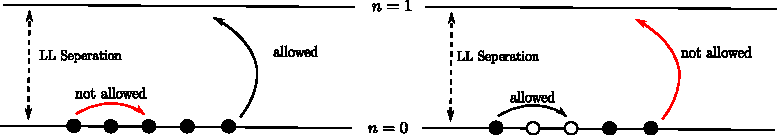
\includegraphics[scale=1.1]{LL.pdf}
			\caption{{\bf Comparison of the Filled and Partially Filled LL}. The \emph{inter-LL} excitation is preferred in the left subgraph due to the Pauli exclusion principle of filled LL, while is suppressed in the right subgraph of partiall filled LL for the higher energy scale of LL seperation comparing with intra-LL interaction.}
			\label{fig:1}
		\end{figure}
		 
		General interactive Hamiltonian in our case takes the form of \cite{nomura2006quantum,goerbig2006electron}
		\begin{equation}\label{0.2.4}
			H_n=\dfrac{1}{2}\sum_{\bm{q}}v_n(\bm{q})\widetilde{\rho}(\bm{-q})\widetilde{\rho}(\bm{q}),  
		\end{equation}
		with the simple effective interaction potential
		\begin{equation*}
			v_n(\bm{q})=\dfrac{2\pi e^2}{\varepsilon|\bm{q}|}\mathcal{F}_n^2(\bm{q}),
		\end{equation*}
		and the former factors
		\begin{equation*}
			\mathcal{F}_n(\bm{q})=\dfrac{1}{2}\left[(1-\delta_{0,n})L_{n-1}\left(\dfrac{q^2\ell_B^2}{2}\right)+(1+\delta_{0,n})L_{n}\left(\dfrac{q^2\ell_B^2}{2}\right)\right]e^{-q^2\ell_B^2/4}.
		\end{equation*}
		But since we focus on the lowest LL $n=0$, the projective Coulomb interaction \eqref{0.2.4} reduces to the familiar form\footnote{We always have $L_0(z)=0$ for the zeroth order of Laguerre polynomial.}
		\begin{equation}\label{0.2.5}
			H_{\text{int}}=\dfrac{1}{2}\sum_{\bm{q}}\dfrac{2\pi e^2}{\varepsilon|\bm{q}|}\widetilde{\rho}(\bm{-q})\widetilde{\rho}(\bm{q}).
		\end{equation}
		Goeribig thought there is no kinetic term in the Hamiltonian for all processes involve merely states within the same LL \cite{goerbig2011electronic}, but we disagree with this claim. 
\iffalse
	\section{}
		\indent\par Attempts of imposing strain on graphene started started from early age. For instance, uniaxial strain is applied to tune the characteristics of Ramann spectrum and open the band grap \cite{ni2008uniaxial,farjam2009comment}. However, it has not aroused much attention until Manes's general revelation of the relation between elastic strain and psuedomagnetic field in monolayer graphene \cite{manes2007symmetry} such that an {\bf arbitrary two-dimensional strain field $u(\bm{r})$ could lead to a pseudo gauge field}
		\begin{equation}\label{1.1.1}
			\bm{A}=\dfrac{t\beta}{ev_F}\left(\begin{array}{c}u_{xx}-u_{yy}\\-2u_{xy}\end{array}\right),
		\end{equation}
		where $t$ is the nearest-neighbor hopping parameter, $\beta=-\partial\ln t/\partial\ln a$ is the dimensionless coupling parameter discribing lattice deformation. And the following Guinea {\it et al.}'s realization of pseudomagnetic QHE \cite{guinea2010energy} without help of the external magnetic fields but this pseudo one, which share similar picture of quantum spin Hall effect (QSHE) \cite{bernevig2006quantum}, pushed this hot spot to new heights. Through imposing an small triangular symmetric strain to a honeycomb lattice, Guinea {\it et al.} construct with an extremely high but nearly uniform psuedomagnetic fields in the Frist Brillouin Zone and propose an experimental methods to achieve that, which is numerically achieved by Verbiest \cite{verbiest2015uniformity}. And what makes it different from the usual situation when high external magnetic field is applied is that this pseudomagnetic field \emph{flips around the two Dirac point}, $K$ and $K'$.\par
		In light of the high pseudomagnetic field and adjustable dopping rate, we believe in the existence of FQHE in strined graphene as well. And the property of massless Dirac fermions and opposite directiton of pseudomagnetic field make the electromagnetic response also valuable to study.
\fi
	\section{Symmetrical Strain on Graphene}
		\indent\par Attempts of imposing strain on graphene started started from early age. For instance, uniaxial strain is applied to tune the characteristics of Ramann spectrum and open the band grap \cite{ni2008uniaxial,farjam2009comment}. However, it has not aroused much attention until Manes's general revelation of the relation between elastic strain and psuedomagnetic field in monolayer graphene \cite{manes2007symmetry} such that an {\bf arbitrary two-dimensional strain field $u(\bm{r})$ could lead to a pseudo gauge field}
		\begin{equation}\label{1.1.1}
			\bm{A}=\dfrac{t\beta}{ev_F}\left(\begin{array}{c}u_{xx}-u_{yy}\\-2u_{xy}\end{array}\right),
		\end{equation}
		where $t$ is the nearest-neighbor hopping parameter, $\beta=-\partial\ln t/\partial\ln a$ is the dimensionless coupling parameter discribing lattice deformation. And the following Guinea {\it et al.}'s realization of pseudomagnetic QHE \cite{guinea2010energy} without help of the external magnetic fields but this pseudo one, which share similar picture of quantum spin Hall effect (QSHE) \cite{bernevig2006quantum}, pushed this hot spot to new heights. Through imposing an small triangular symmetric strain to a honeycomb lattice, Guinea {\it et al.} construct with an extremely high but nearly uniform psuedomagnetic fields in the Frist Brillouin Zone and propose an experimental methods to achieve that, which is numerically achieved by Verbiest \cite{verbiest2015uniformity}. And what makes it different from the usual situation when high external magnetic field is applied is that this pseudomagnetic field \emph{flips around the two Dirac point}, $K$ and $K'$.\par
		In light of the high pseudomagnetic field and adjustable dopping rate, we believe in the existence of FQHE in strined graphene as well. And the property of massless Dirac fermions and opposite directiton of pseudomagnetic field make the electromagnetic response also valuable to study.
		
\chapter{SU(2) Fermionic Chern-Simons Field Theory of Non-relativistic Fermions in Graphene}
	\section{Discussion on the Effective Hamiltonian}
		\indent\par 
		\iffalse
			To sum up, in our case the free part of the massless Dirac fermion in graphene is now dominated by the second quantized Hamiltonian
			\begin{equation}\label{1.1.2}
				H_0=\sum_{\alpha}\sum_{\bm{p}}(\psi_e)_\alpha^\dagger (-1)^\alpha v_F\bm{\sigma}\cdot(\bm{p}+(-1)^\alpha e\bm{A})(\psi_e)_\alpha,
			\end{equation}
			where $a=1,2,3,4$ represent the sublattice and valley degenerancy such that the eigenstate is chosen in the order $(\psi_e)_\alpha\equiv\left((\psi_e)_{K\uparrow}, (\psi_e)_{K'\uparrow}, (\psi_e)_{K\downarrow}, (\psi_e)_{K'\downarrow}\right)$. The subscripts $e$ is still introduced to distinguish the field operators of massless Dirac fermions with those of composite Dirac fermions. But the RG flow analysis conducted by Sheely {\it et al.} in \cite{sheehy2007quantum} revealed that, Coulomb interaction also plays a significant role near the quantum cirtical point in graphene. Therefore the whole Hamiltonian takes the form of
			\begin{equation}\label{1.1.3}
				H=\sum_{\alpha}\sum_{\bm{p}}(\psi_e)_\alpha^\dagger(-1)^\alpha v_F\bm{\sigma}\cdot(\bm{p}+(-1)^\alpha e\bm{A})(\psi_e)_\alpha+\dfrac{1}{2}\sum_{\alpha,\alpha'}(\psi_e)_\alpha^\dagger(\psi_e)_{\alpha'}^\dagger v(q) (\psi_e)_{\alpha'}(\psi_e)_{\alpha}.
			\end{equation}
		\fi
		Theorefore our system is similar to the same as the non-relativistic bilayer system studied by both Lopez and Fradkin in \cite{lopez1995fermionic,rajaraman1997generalized}. And the second quantized Hamiltonian takes the form of (for convenience of the following computation of electromagnetic response, apart from the external magnetic field $\bm{A}$ appiled, we also write down the probing pseudo-magnetic field $\bm{A'}$ explicitly, which results from the symmetrical strained graphene and thus \emph{alters its direction} for different valley index)
		\begin{align}\label{2.1.1}
			H&=\sum_\alpha\int\dd^3x\,(\psi_e)^\dagger_\alpha(x)\dfrac{1}{2m}\left(-i\nabla+e\bm{A}+e\bm{A'}^\alpha\right)^2(\psi_e)_\alpha(x)\nonumber\\
			&\qquad+\dfrac{1}{2}\sum_{\alpha \beta}\int\dd^3x\dd^3x'\,\delta(\hat{\rho}_e)_\alpha(x)v_{\alpha \beta}(|\bm{x}-\bm{x'}|)\delta(\hat{\rho}_e)_\beta(x'),
		\end{align}
		where 
		\begin{equation*}
			\bm{A'}^\alpha=\begin{cases}
				+\bm{A'},&\alpha=\uparrow,\\
				-\bm{A'},&\alpha=\downarrow,
			\end{cases}
		\end{equation*}
		the fluctuation of charge density $\delta\hat{(\psi_e)}(x)_a\equiv(\psi_e)^\dagger_\alpha(x)(\psi_e)_\alpha(x)-(\bar{\rho}_e)_\alpha(x)$, and the Coulomb interaction $v(|r|)=\frac{e^2}{\varepsilon |r|}$.
	\section{Introduction of Chern-Simons Fields and K-matrix}
		\indent\par Similar to the situation in HLR, we take the \emph{singular unitary transformation} $\psi_\alpha\mapsto(\psi_e)_\alpha=U_\alpha(\psi_e)_\alpha$ to transfer our strongly-correlated system to an equivalent one but easy to handle with. And in light of the increase of freedom of our field operator, the unitary operator should be generalized to 
		\begin{equation}\label{2.2.1}
			U_\alpha\equiv\exp \left[i\mathcal{K}^{\alpha \beta}\int\dd\bm{r'}\,\mathrm{arg}(\bm{r}-\bm{r'})\rho_\beta(\bm{r'}) \right]
		\end{equation}
		in our situation, where the function $\mathrm{arg}(\bm{r}-\bm{r'})\equiv\arctan\frac{y-y'}{x-x'}$ and Einstein's summation rule of repeated greek indices $\alpha,\beta=\uparrow,\downarrow$ is implemented. The $\mathcal{K}$-matrix introduced by Wen and Zee in [???] should take the form of \cite{mandal1996theory}
		\begin{equation}\label{2.2.2}
			\mathcal{K}^{\alpha \beta}=\left(\begin{array}{cc}
				2k_1 & m \\ m & 2k_2
			\end{array}\right) 
		\end{equation}
		since the proof of equivalence proposed by Lopez and Fradkin in \cite{lopez1991fractional} can be safely generalized to higher freedoms.\par
		Again define the vector fields
		\begin{equation}\label{2.2.3}
			e\bm{a}^\alpha(\bm{r})=\mathcal{K}^{\alpha \beta}\int\dd\bm{r'}\,\nabla\mathrm{arg}(\bm{r}-\bm{r'})\rho_\beta(\bm{r'})=\mathcal{K}^{\alpha\beta}\int\dd\bm{r'}\,\dfrac{\varepsilon_{ij}(\bm{r}_i-\bm{r'}_j)}{|\bm{r}-\bm{r'}|}\rho_\beta(\bm{r'}),
		\end{equation}
		then clearly the orignal Hamiltonian is equivalent to the system with new Chern-Simons gauge fields $\bm{a}^\alpha$ included\footnote{Note that the singular unitary transformation does not change the form of density operator.}
		\begin{align}\label{2.2.4}
			H&=\sum_\alpha\int\dd^3x\,\psi^\dagger_\alpha(x)\dfrac{1}{2m}\left(-i\nabla+e\bm{A}+e\bm{A'}^\alpha-e\bm{a}^\alpha\right)^2\psi_\alpha(x)\nonumber\\
			&\qquad+\dfrac{1}{2}\sum_{\alpha \beta}\int\dd^3x\dd^3x'\,\delta\hat{\rho}_\alpha(x)v{\alpha \beta}(|\bm{x}-\bm{x'}|)\delta\hat{\rho}_\beta(x').
		\end{align}
		So apart from the external magnetic fields we impose before, each electron at position $\bm{r}$ is now attached with several other magentic flux
		\begin{equation}\label{2.2.5}
			\bm{B}^\alpha_{\text{CS}}\equiv\nabla\times\bm{a}^\alpha=-\dfrac{2\pi}{e}\mathcal{K}^{\alpha \beta}\rho_\beta(\bm{r}).
		\end{equation}
		The accurate number of flux cannot be determined in this theory, but in light of the \emph{Marginal Fermi-liquid} half-filling FQHE state studied by \cite{Halperin1995Theory} in monolayer system, we also believe the existence of Fermi-liquid-like state $\nu=1/2$ in graphene. In HLR's motivation, {\bf the external magnetic field felt by an arbitrary fermion is accurately eliminated by the Chern-Simons magnetic field}, viz
		\begin{equation}\label{2.2.6}
			\bm{B}^\alpha_{\text{eff}}\equiv\bm{B}_{\text{ext}}+\bm{B}^\alpha_{\text{CS}}=0.
		\end{equation}
		but with a much more suble physical picture here since {\bf the attached flux of electrons in one band will certainly influence the electrons in the other band as well, and vice versa}.\par
		Duality of two valley degenerancy of graphene, $K$ and $K'$, guarantees that the number of electrons in each freedom is \emph{the same} (and approximately conserved) $N_1=N_2=N/2$ and subject to the same strenght of external magnetic fields, or attach the same number of Chern-Simons magnetic flux to compensate the external magnetic fields. Therefore, it's reasonable to have $\nu_\alpha=\frac{(\rho_e)_{\alpha}S}{BS/\phi_0}=\frac{\nu}{2}=\frac{1}{4}$, which can be realized if the $\mathcal{K}-$matrix is chosen as the \emph{invertible} form
		\begin{equation}\label{2.2.7}
			\mathcal{K}^{\alpha \beta}=\left(\begin{array}{cc}
				\widetilde{\phi}  & \widetilde{\phi}  \\ \widetilde{\phi}  & \widetilde{\phi} 
			\end{array}\right)
		\end{equation}
		with $\widetilde{\phi}=2$. And all the following computation bases on this assuming matrix.
	\section{Action of Fermionic Chern-Simons Theory}
		\indent\par After bringing in the Chern-Simons field in $\nu=\frac{1}{2}$ FQHE system, composite fermions subjected to \emph{zero} effective magnetic field are now govened by the new Hamiltonian \eqref{2.2.4} as well as the \emph{constraint conditions} \eqref{2.2.5} and \eqref{2.2.6}, which, are actually the dynamical equation of Chern-Simons field $\bm{a}^\alpha$. And it is because of our choice of invertible $\mathcal{K}-$matrix that leads to the degenerancy of one of the Chern-Simons field  since from \eqref{2.2.5} and \eqref{2.2.6} we always have $\bm{a}^\uparrow\equiv \bm{a}^\downarrow$. And from now on we will omit the valley index of Chern-Simons field, simply writting it as $\bm{a}$ instead.\par
		Working in \emph{Coulomb gauge}, i.e., $\nabla\cdot \bm{a}=\nabla\cdot\bm{A}=\nabla\cdot\bm{A'}^\alpha=0$, then $a_{||}(p)=A_{||}(p)={A'}^\alpha_{||}(p)=0$ if we decompose them into \emph{transverse} and \emph{longtitudinal} components (write in momentum space)\footnote{By Helmholz theorem (or Hodge Decomposition), any arbitrary field can be decomposed by an irrotational field and a solenoidal field. Coulomb gauge equation $\nabla\cdot\bm{a}=0$ is equivalent to $a_{||}=0$, since in momentum space
		\begin{equation*}
			\bm{p}\cdot\bm{a}=\dfrac{p_i p^i}{|\bm{p}|}_{||}+\dfrac{\varepsilon_{ij}p^jp^i}{|\bm{p}|}a_{\perp}=\dfrac{p_i p^i}{|\bm{p}|}a_{||}=0\implies a_{||}=0.
		\end{equation*}}
		\begin{equation}\label{2.3.0}
			a_i(p)\equiv\dfrac{p_i}{|\bm{p}|}a_{||}(p)+\dfrac{\varepsilon_{ij}p^j}{|\bm{p}|} a_{\perp}(p).
		\end{equation}
		Certainly gauge fixing could also be done after obtaining the action below, and the standard Fadeev-Popov method in high energy physics is introduced to accomplish this, cf \cite{peskin1995introduction} for details.\par
		For the future unified treatment of Gaussian fluctuation, it is better to recover the dynamical equation of $\bm{a}$ back into the action such that in coherent state path integral formalism the partition function can be extended to both fermionic fields and Chern-Simons fields (in imaginary time $t\equiv-i\tau$)
		\begin{align}
			\mathcal{Z}&=\int \mathcal{D}(\bar{\psi}_\uparrow,\psi_\uparrow)\mathcal{D}(\bar{\psi}_\downarrow,\psi_\downarrow)\,e^{-S[\bar{\psi}_\uparrow,\psi_\uparrow,\bar{\psi}_\downarrow,\psi_\downarrow]}\nonumber\\
			&=\int\mathcal{D}(\bar{\psi}_\uparrow,\psi_\uparrow)\mathcal{D}(\bar{\psi}_\downarrow,\psi_\downarrow)\mathcal{D}a_{\perp}\,\prod_{\bm{x},\tau}\delta\left(B_{\text{CS}}+\phi_0\widetilde{\phi}(\rho^\uparrow+\rho^\downarrow)\right)\,e^{-S[\bar{\psi}_\uparrow,\psi_\uparrow,\bar{\psi}_\downarrow,\psi_\downarrow,a_\perp]}\nonumber\\
			&=\mathcal{Z}_0\int\mathcal{D}(\bar{\psi}_\uparrow,\psi_\uparrow)\mathcal{D}(\bar{\psi}_\downarrow,\psi_\downarrow)\mathcal{D}a_0\mathcal{D}a_{\perp}\nonumber\\
			&\qquad\exp \bigg\{-\int_0^\beta\dd\tau\int\dd\bm{x}\,\left(\dfrac{\varepsilon^{ij}\partial_i a_j}{\phi_0\widetilde{\phi}}+\rho_\uparrow+\rho_\downarrow\right)a_0-S[\bar{\psi}_\uparrow,\psi_\uparrow,\bar{\psi}_\downarrow,\psi_\downarrow,a_\perp]\bigg\}\nonumber\\
			&=\mathcal{Z}_0\int\mathcal{D}(\bar{\psi}_\uparrow,\psi_\uparrow)\mathcal{D}(\bar{\psi}_\downarrow,\psi_\downarrow)\mathcal{D}a_0\mathcal{D}a_{\perp}\nonumber\\
			&\qquad\exp \left\{-S_{\text{CF}}[\bar{\psi},\psi,a_0,a_{\perp}]-S_{\text{int}}[\bar{\psi},\psi]-S_{\text{CS}}[a_0,a_{\perp}]\right\},\label{2.3.1}
		\end{align}
		where in the first line we insert a functional version of the integral over Dirac delta function\footnote{Taking the concrete definition of path integral into account helps understand this identity as infinite multiplication of usual Lebesgue integral over the generalized function space
		\begin{equation*}
			\mathds{1}=\lim_{N\rightarrow \infty}\prod_{k=0}^N\int\dd a_{\perp}(x_k)\,\delta(\varepsilon^{ij} \partial_i a_j(x_k)+\phi_0 \mathcal{K}^{\alpha \beta}\rho_{\beta}(x_k,t_k) ).
		\end{equation*}}
		\begin{equation*}
			\mathds{1}\equiv\int\mathcal{D}a_{\perp}\prod_{\bm{x},\tau}\delta(\varepsilon^{ij}\partial_i a_j+\phi_0\mathcal{K}^{\alpha \beta}\rho_\beta(\bm{x},\tau)),
		\end{equation*}
		in the second line we first extract the common factor $\phi_0\widetilde{\mathcal{K}}$, which gives an irrelevant normalization factor $\mathcal{Z}_0$, then perform a \emph{functional version of Fourier Transformation} of Dirac delta function\footnote{The Chern-Simons gauge field we brought in before is just of \emph{two-component}. So this functional Fourier Transformation should be regarded as the \emph{definition} of $a_0$. We write them together just for convenience.} with the dual function donoted as $a_0(\bm{x},\tau)$
		\begin{equation*}
			\prod_{\bm{x},\tau}\delta\left(\dfrac{\varepsilon^{ij}\partial_i a_j}{\phi_0 \widetilde{\phi} }+\rho_\uparrow+\rho_\downarrow\right)\equiv\int \mathcal{D}a_0\,\exp \left(-\int_0^\beta\dd\tau\int\dd^2 x\,a_0\left(\dfrac{\varepsilon^{ij}\partial_i a_j}{\phi_0\widetilde{\phi}} +\rho_\uparrow+\rho_\downarrow\right) \right),
		\end{equation*}
		and in the third line we re-arrange terms and divide them into three parts
		\begin{itemize}
		\item the action of composite fermion 
			\begin{align}\label{2.3.2}
				S_{\text{CF}}[\bar{\psi},\psi,a_0,a_{\perp}]&=\sum_\alpha\int_0^\beta\dd\tau\int\dd^2 x\,\bar{\psi}_\alpha\bigg[\partial_\tau+\mu-a_0+\nonumber\\
				&\qquad\dfrac{1}{2m}(-i\nabla+e\bm{A}+e\bm{A'}^\alpha+e\bm{a})^2\bigg]\psi_\alpha,
			\end{align}
		\item the action of interacting composite fermions 
			\begin{align}\label{2.3.3}
				S_{\text{int}}[\bar{\psi},\psi]&=\sum_{\alpha \beta}\dfrac{1}{2}\int_0^\beta\dd\tau\dd\tau'\int\dd^2 x\dd^2 x'\nonumber\\
				&\qquad(\bar{\psi}_\alpha(\bm{x})\bar{\psi}_\alpha(\bm{x})-\bar{\rho}_\alpha)v(\bm{x}-\bm{x'})(\bar{\psi}_\beta(\bm{x'})\psi_\beta(\bm{x})-\bar{\rho}_\beta),
			\end{align}
		\item and the action of Chern-Simons field
			\begin{equation}\label{2.3.4}
				S_{\text{CS}}[a_0,a_{\perp}]=\dfrac{1}{\phi_0\widetilde{\phi}}\int_0^\beta\dd\tau\int\dd^2 x\,a_0 \varepsilon^{ij}\partial_i a_j.
			\end{equation}
		\end{itemize}
		And by Coulomb gauge we can simplify \eqref{2.3.2} by expanding the parentheses
		\begin{align}
			S_{\text{CF}}&=\sum_\alpha\int_0^\beta\dd\tau\int\dd^2x\,\bar{\psi}_\alpha\bigg[\partial_\tau+\mu-a_0-\dfrac{1}{2m}\nabla^2-\dfrac{ie}{2m}\nabla\cdot(\bm{A}+\bm{A'}^\alpha+\bm{a})\nonumber\\
			&\qquad-\dfrac{ie}{2m}(\bm{A}+\bm{A'}^\alpha+\bm{a})\cdot\nabla+\dfrac{e^2}{2m}(\bm{A}+\bm{A'}^\alpha+\bm{a})^2\bigg]\psi_\alpha\nonumber\\
			&=\sum_\alpha\int_0^\beta\dd\tau\int\dd^2x\,\bar{\psi}_\alpha\bigg[\mathcal{G}_0^{-1}+\hat{\chi}^\alpha_1+\hat{\chi}^\alpha_2\bigg]\psi_\alpha,\label{2.3.5}
		\end{align}
		where
		\begin{equation*}
			\hat{\mathcal{G}}_0=\left(\partial_\tau+\mu-\dfrac{1}{2m}\nabla^2\right)^{-1},\quad \hat{\chi}^\alpha_1\equiv -a_0-\dfrac{ie}{m}(\bm{A}+\bm{A'}^\alpha+\bm{a})\cdot\nabla,\quad \hat{\chi}^\alpha_2=\dfrac{e^2}{2m}(\bm{A}+\bm{A'}^\alpha+\bm{a})^2.
		\end{equation*}
		Therefore, the partition function can be obtained if we integrate out all freedoms, which are dominated by the above three parts of actions.
	
	\section{Mean-field Approximation and Gaussian Fluctuation}
		\indent\par In this section, we first derive the effection action of gauge field $a_\mu(\bm{x})$ as Lopez and Fradkin them did in \cite{lopez1991fractional}. Subsequently we will expand the effective action to the second order to obtain the Gaussian fluctuation around the mean-field.\par
		Due to the \emph{quartic} form of Coulomb interaction, an direct integration over fermionic operators to obtain the effective action of Chern-Simons field is not readily possible. In fact, a \emph{Hubbard-Stratonovich Transformation} of density-density channel has to be performed before the integration to reduce the power of fermionic operators. Through introducing an auxiliary bosonic operator and shifting it to eliminate the quartic interaction, we are left with a \emph{quardratic} form of this auxiliary field, which can be integrated out standardly with Gauss integral formula \cite{Stratonovich1957On,hubbard1959calculation,altland2010condensed}.\par
		However, since the dynamic equation \eqref{2.2.5} and \eqref{2.2.6} exactly connect Chern-Simons field with fermionic field, this standard procedure can be circumvented by simple substitution of $\psi$ with $\bm{a}$, giving
		\begin{equation}\label{2.4.1}
			S_{\text{int}}=\dfrac{1}{2}\int\dd^3 x\dd^3 x' \left(\dfrac{\varepsilon^{ij}\partial_i a_j(\bm{x})}{2\widetilde{\phi}\phi_0}-\bar{\rho}\right) v(\bm{x}-\bm{x'})\left(\dfrac{\varepsilon^{k\ell}\partial_k a_\ell(\bm{x'})}{2\widetilde{\phi}\phi_0}-\bar{\rho}\right).
		\end{equation}
		\indent Now that the left parts of action in \eqref{2.3.1}, i.e. the action of composite fermions \eqref{2.3.5}, is of quardratic form, then the effective action of bosonic operators can be obtained by integrate out all fermionic freedoms as following
		\begin{align}
			S_{\text{CF-eff}}[a_0,a_{\perp}]&=\sum_\alpha\ln\mathrm{det}\left[\hat{\mathcal{G}}_0^{-1}+\hat{\chi}^\alpha_1+\hat{\chi}^\alpha_2\right]=\sum_\alpha\mathrm{tr}\ln\left[\hat{\mathcal{G}}_0^{-1}+\hat{\chi}^\alpha_1+\hat{\chi}^\alpha_2\right]\nonumber\\
			&=2\mathrm{tr}\left(\ln\hat{\mathcal{G}}_0^{-1}\right)+\sum_\alpha\mathrm{tr}\left(\hat{\mathcal{G}}_0\hat{\chi}^\alpha_1\right)+\sum_\alpha\mathrm{tr}\left(\hat{\mathcal{G}}_0\hat{\chi}^\alpha_2+\dfrac{1}{2}\hat{\mathcal{G}}_0\hat{\chi}^\alpha_1\hat{\mathcal{G}}_0\hat{\chi}^\alpha_1\right)\nonumber\\
			&\quad+\mathcal{O}(|a_0|^3,|\bm{a}|^3).\label{2.4.2}
		\end{align}
		The first term is irrelevant to all bosonic freedoms so can be absorbed in $\mathcal{Z}_0$. The second term also vanishes since we expand around the saddle-point $a_\mu: \bar{a}_\mu\mapsto \bar{a}_\mu+a_\mu$, with $\bar{a}_\mu$ subject to the \emph{mean-field equation} \eqref{2.2.5}
		\begin{equation}\label{2.4.3}
			\varepsilon^{ij}\partial_i \bar{a}_j^\alpha=-\dfrac{2\pi}{e}\mathcal{K}^{\alpha \beta}\bar{\rho}_\beta(\bm{x}),
		\end{equation}
		which is in conformity with the requirment of a vanishing first variation\footnote{Perturbation must comply with the gauge condition of the Chern-Simons fields. So $a_{||}, A_{||}$ and $A'_{||}$ stay to be zero all the time.}
		\begin{align*}
			\dfrac{\delta S}{\delta a_i}\bigg|_{\substack{\bar{a}_0=0\\\varepsilon^{ij}\partial_i\bar{a}_j=-2\phi_0\widetilde{\phi}\bar{\rho}}}&=\dfrac{\delta S_{\text{CF-eff}}}{\delta a_i}+\dfrac{\delta S_{\text{int}}}{\delta a_i}+\dfrac{\delta S_{\text{CS}}}{\delta a_i}\\
			&=-\dfrac{1}{2}\int\dd^3 x\dd^3 x' \bar{\rho}v(\bm{x}-\bm{x'})\left(\dfrac{\varepsilon^{k\ell}\partial_k \bar{a}_\ell(\bm{x'})}{2\widetilde{\phi}\phi_0}-\bar{\rho}\right)=0.
		\end{align*}
		So the first non-trivial term contributing to electromagnetic linear reponse is the second order expansion of \eqref{2.4.2}.\par
		Given the gauge conditioin \eqref{2.3.0} we chose, it's more convenient to simplify the trace in momentum space instead. So we start with re-expressing the action of composite fermions as following
		\begin{equation}\label{2.4.4}
			S_{\text{CF}}=\sum_\alpha\sum_{\bm{q}_1,\omega_n}\sum_{\bm{q}_2,\omega_m}\,\bar{\psi}_{\alpha,q_1}\bigg[(\hat{\mathcal{G}}_0^{-1})_{q_1,q_2}+(\hat{\chi}^\alpha_1)_{q_1,q_2}+(\hat{\chi}^\alpha_2)_{q_1,q_2}\bigg]\psi_{\alpha,q_2},
		\end{equation} 
		where\footnote{Results here is straight to verify. The notation $(\hat{\mathcal{G}}_0^{-1})_{q_1,q_2}$ in \eqref{2.4.5a}, for instance, is a conventional notation representing a matrix element in momentum space \cite{altland2010condensed,nagaosa2013quantum}.}
		\begin{subequations} % label subequations as (15a) (15b)2
		\begin{align}
			(\hat{\mathcal{G}}_0^{-1})_{q_1,q_2}&\equiv \mathcal{G}_0^{-1}(\bm{q}_1,i\omega_n)\delta_{\bm{q}_1,\bm{q}_2}\delta_{\omega_n,\omega_m},\label{2.4.5a}\\
			(\hat{\chi}^\alpha_1)_{q_1,q_2}&\equiv-a_0(q_1-q_2)-\dfrac{e}{m}\bigg(\bm{a}+\bm{A}+\bm{A'}^\alpha\bigg)(q_1-q_2)\cdot \bm{q}_2,\label{2.4.5b}\\
			(\hat{\chi}^\alpha_2)_{q_1,q_2}&\equiv\dfrac{e^2}{2m}\sum_{q}\bigg(\bm{a}+\bm{A}+\bm{A'}^\alpha\bigg)(q+q_1)\cdot \bigg(\bm{a}+\bm{A}+\bm{A'}^\alpha\bigg)(-q-q_2)\label{2.4.5c}.
		\end{align}
		\end{subequations}
		\indent Still integrating out the fermionic operators and expanding around saddle point, the first part of the trace now can be shown as
		\begin{align}\label{2.4.6}
			\mathrm{tr}\left(\hat{\mathcal{G}}_0\hat{\chi}^\alpha_2\right)&=\sum_p(\mathcal{G}_0)_p (\chi^\alpha_2)_{p,p}=\dfrac{e^2}{2m}\sum_{p,q}(\mathcal{G}_0)_p(\bm{a}+\bm{A'}^\alpha)_{p+q}\cdot(\bm{a}+\bm{A'}^\alpha)_{-p-q}\nonumber\\
			&=\dfrac{e^2}{2m}\sum_{p,q}(\mathcal{G}_0)_p\dfrac{\varepsilon^{ij}(p^i+q^i)}{|\bm{p}+\bm{q}|}(a_{\perp}+{A'}^\alpha_\perp)_{p+q}\dfrac{\varepsilon_{ik}(-p^k-q^k)}{|\bm{p}+\bm{q}|}(a_{\perp}+{A'}^\alpha)_{-p-q}\nonumber\\
			&=\sum_q(a_{\perp}+{A'}^\alpha_\perp)_{-q}\left(\dfrac{e^2}{2m}\sum_p(\mathcal{G}_0)_p\right)(a_{\perp}+{A'}^\alpha_\perp)_{q}\nonumber\\
			&=\sum_q(a_{\perp}+{A'}^\alpha_\perp)_{-q}\left(-\dfrac{e^2n_e}{2m}\right)(a_{\perp}+{A'}^\alpha_\perp)_{q},
		\end{align}
		where in the last line we shift the integral variable $q$ by $-p$ and substitute the identity
		\begin{align*}
			\sum_{\bm{p},\omega_n} \mathcal{G}_0(\bm{p},i\omega_n)&=\lim_{\tau \rightarrow 0}\sum_{\bm{p},\omega_n}e^{-i\omega_n \tau} \mathcal{G}_0(\bm{p},i\omega_n)=\lim_{\tau\rightarrow 0}\sum_{\bm{p}}\mathcal{G}_0(\bm{p},\tau)\equiv\lim_{\tau \rightarrow 0}\sum_{\bm{p}}\langle T_\tau\psi(\bm{p},\tau)\psi^\dagger(\bm{p},\tau)\rangle\nonumber\\
			&=-\sum_{\bm{p}}\langle\psi^\dagger(\bm{p})\psi(\bm{p})\rangle=-\sum_{\bm{p}}\hat{\rho}(\bm{p})=-n_F(\xi_{\bm{p}}).
		\end{align*}
		The second part of the trace is much more tedious
		\begin{align}
			\mathrm{tr}\left(\dfrac{1}{2}\hat{\mathcal{G}}_0\hat{\chi}^\alpha_1\hat{\mathcal{G}}_0\hat{\chi}^\alpha_1\right)&=\dfrac{1}{2}\sum_{p,q}(\mathcal{G}_0)_p (a_0+{A'}^\alpha_0)_{p,q} (\mathcal{G}_0)_q (a_0+{A'}^\alpha_0)_{q,p}\nonumber\\
			&+\dfrac{1}{2}\sum_{p,q}(\mathcal{G}_0)_{p}(a_0+{A'}_0^\alpha)_{p,q}(\mathcal{G}_0)_{q} \left(\dfrac{e}{m}(\bm{a}+\bm{A'}^\alpha)\cdot\bm{p}\right)_{q,p}\nonumber\\
			&+\dfrac{1}{2}\sum_{p,q}(\mathcal{G}_0)_{p}\left(\dfrac{e}{m}(\bm{a}+\bm{A'}^\alpha)\cdot\bm{p}\right)_{p,q}(\mathcal{G}_0)_{q}(a_0+{A'}^\alpha_0)_{q,p}\nonumber\\
			&+\dfrac{1}{2}\sum_{p,q}(\mathcal{G}_0)_{p}\left(\dfrac{e}{m}(\bm{a}+\bm{A'}^\alpha)\cdot\bm{p}\right)_{p,q}(\mathcal{G}_0)_{q}\left(\dfrac{e}{m}(\bm{a}+\bm{A'}^\alpha)\cdot\bm{p}\right)_{q,p}\nonumber\\
			%&=\dfrac{1}{2}\sum_{p,q}(a_0)_{p-q}\cdot(\mathcal{G}_0)_p(\mathcal{G}_0)_q\cdot(a_0)_{q-p}+\dfrac{1}{2}\sum_{p,q}(a_0)_{p-q}\cdot(\mathcal{G}_0)_p (\mathcal{G}_0)_{q}\dfrac{ep_i}{m}\dfrac{\varepsilon^{ij}(q_j-p_j)}{|\bm{q-p}|}\cdot(a_\perp)_{q-p}\nonumber\\
			%&\qquad+\dfrac{1}{2}\sum_{p,q}(a_\perp)_{p-q}\cdot(\mathcal{G}_0)_p (\mathcal{G}_0)_{q}\dfrac{eq_i}{m}\dfrac{\varepsilon^{ij}(q_j-p_j)}{|\bm{q-p}|}\cdot(a_0)_{q-p}\nonumber\\
			%&\qquad+\dfrac{1}{2}\sum_{p,q}(a_\perp)_{p-q}\cdot\dfrac{\varepsilon^{ij}(p_j-q_j)}{|\bm{p}-\bm{q}|}\dfrac{ep_i}{m}(\mathcal{G}_0)_{p}(\mathcal{G}_0)_{q}\dfrac{ep_l}{m}\dfrac{\varepsilon^{kl}(p_l-q_l)}{|\bm{p}-\bm{q}|}\cdot(a_\perp)_{q-p}\nonumber\\
			&=\dfrac{1}{2}\sum_{p,q}(a_0+{A'}^\alpha_0)_{-q}\cdot(\mathcal{G}_0)_p(\mathcal{G}_0)_{p+q}\cdot(a_0+{A'}^\alpha_0)_{q}\nonumber\\
			&+\dfrac{1}{2}\sum_{p,q}(a_0+{A'}^\alpha_0)_{-q}\cdot(\mathcal{G}_0)_p (\mathcal{G}_0)_{p+q}\dfrac{ep_i}{m}\dfrac{\varepsilon^{ij}q_j}{|\bm{q}|}\cdot(a_\perp+{A'}^\alpha_\perp)_{q}\nonumber\\
			&+\dfrac{1}{2}\sum_{p,q}(a_\perp+{A'}^\alpha_\perp)_{-q}\cdot(\mathcal{G}_0)_p (\mathcal{G}_0)_{q+p}\dfrac{ep_i}{m}\dfrac{\varepsilon^{ij}q_j}{|\bm{q}|}\cdot(a_0+{A'}^\alpha_0)_{q}\nonumber\\
			&+\dfrac{1}{2}\sum_{p,q}(a_\perp+{A'}^\alpha_\perp)_{-q}\cdot\dfrac{\varepsilon^{ij}(-q_j)}{|\bm{q}|}\dfrac{ep_i}{m}(\mathcal{G}_0)_{p}(\mathcal{G}_0)_{p+q}\dfrac{ep_l}{m}\dfrac{\varepsilon^{kl}q_l}{|\bm{q}|}\cdot(a_\perp+{A'}^\alpha_\perp)_{q},\label{2.4.7}
		\end{align}
		where in the second equal sign we shift the variable $q$ to $q\mapsto p+q$ as well.\par
		In Halperin {\it et al.}'s work \cite{Halperin1995Theory}, they ignore the off-diagnal terms, viz the second and third terms in \eqref{2.4.7}, under the \emph{Long wave-length limit} $|q|\ll1$, for $(\mathcal{G}_0)_{p+q}(\mathcal{G}_0)_p\sim(\mathcal{G}_0)_p^2$ is even in momentum, cf. Appendix B for a detailed proof. However, such extreme condition makes our derivation lose generality. So instead, we will follow the lengthy derivation of Lopez and Fradkin to obtain the general expression of \emph{polarization tensor} $\Pi^{\mu \nu}$ such that
		\begin{equation}\label{2.4.6}
			S_{\text{CF}}=\dfrac{1}{2}\sum_{\alpha=\uparrow,\downarrow}\sum_{\mu,\nu}^{0,1}\sum_{\bm{q},\omega_n}\left(a_\mu+{A'}_\mu^\alpha\right)_{-q}\Pi^{\mu\nu}\left(a_\mu+{A'}_\mu^\alpha\right)_{q},
		\end{equation}
		with
		\begin{equation}\label{2.4.7}
			\Pi^{\mu\nu}(\bm{q},i\omega_n)\equiv \left(\begin{array}{cc}
				\displaystyle\sum_p(\mathcal{G}_0)_p(\mathcal{G}_0)_{p+q} & \displaystyle\dfrac{e \varepsilon^{ij} q_j}{m|\bm{q}|}\sum_{p}p_i(\mathcal{G}_0)_p(\mathcal{G}_0)_{p+q}\\
				\displaystyle\dfrac{e \varepsilon^{ij} q_j}{m|\bm{q}|}\sum_{p}p_i(\mathcal{G}_0)_p(\mathcal{G}_0)_{p+q} & \displaystyle-\dfrac{e^2n_e}{m}+\sum_p\dfrac{e^2p^2}{m^2}(\mathcal{G}_0)_p(\mathcal{G}_0)_{p+q}
			\end{array}\right),
		\end{equation}
		as is shown above. Each martix element of $\Pi^{\mu \nu}$ is discussed under distinct extreme conditions in Appendix B and C. But without loss of generality, here we will utilize the \emph{Kallen Lehmann spectrum decomposition theorem} \cite{abrikosov2012methods,peskin1995introduction} to expand the Green function in basis of Landau wave function and express the polarization tensor by lengthy infinite series.\par
		Gauge invariance of the effective action results in the transversity of polarization tensor \cite{Fradkin2013Field}, i.e.,
		\begin{equation}\label{2.4.8}
			\partial_\mu^x\Pi^{\mu\nu}(x,y)=0.
		\end{equation}
		So it is possible to factorize the the polarization tensor into three scalar components, $\Pi^0_\alpha, \Pi^1_\alpha, \Pi^2_\alpha$ \cite{lopez1991fractional,lopez1995fermionic}, reading ($i,j=1,2$ represent $x,y$ component)
		\begin{subequations}
		\begin{align}
			\Pi_\alpha^{00}(\bm{q},\omega)&=-\bm{q}^2\Pi^0_\alpha(\bm{q},\omega),\label{2.4.9a}\\
			\Pi_\alpha^{0i}(\bm{q},\omega)&=-\omega q^i\Pi^0_\alpha(\bm{q},\omega)+i \varepsilon^{0ij}q_j\Pi^1_\alpha(\bm{q},\omega),\label{2.4.9b}\\
			\Pi_\alpha^{i0}(\bm{q},\omega)&=-\omega q^i\Pi^0_\alpha(\bm{q},\omega)-i \varepsilon^{0ij}q_j\Pi^1_\alpha(\bm{q},\omega),\label{2.4.9c}\\
			\Pi_\alpha^{ij}(\bm{q},\omega)&=-\omega^2\delta^{ij}\Pi^0_\alpha(\bm{q},\omega)+i \varepsilon^{0ij}\omega\Pi^1_\alpha(\bm{q},\omega)+(\delta^ij-q^iq^j)\Pi^2_\alpha(\bm{q},\omega),\label{2.4.9d}
		\end{align}
		\end{subequations}
		with the scalar tensor given in the Appendix B of \cite{lopez1991fractional}.

	\section{Electromagnetic Response Tensor and Hall Conductance}
		\indent\par In order to obtain the electromagnetic response tensor 
		\begin{equation*}
			K_{\mu\nu}(x,y):=\frac{\delta^2}{\delta A'_\mu(x)\delta A'_\nu(y)}\ln\mathcal{Z}[\bm{A'}],
		\end{equation*}
		we need to integrate out the residue freedom of statistical field $a_\mu$ in the effective action. Ditto for the Fourier transformation we performed in the previous section to expressed the action of composite fermions in an explicit form \eqref{2.4.6}, the same procedure should be applied with other parts of action. We rexpress the action of Chern-Simons field\footnote{The Fourier transfromed Chern-Simons action is symmetrically splitted
		\begin{align*}
			\int\dd\tau\int\dd^x\,a_0 \varepsilon^{ij}\partial_i a_j&=\sum_{\bm{p},\omega_n}\sum_{\bm{q},\zeta_n}a_0(\bm{p},i\omega_n)\varepsilon^{ij}p_i a_j(\bm{q},i\zeta_n)\delta(\omega_n+\zeta_n)\delta(\bm{p}+\bm{q})\\
			&=\dfrac{1}{2}\sum_{\bm{q},\zeta_n}a_0(-\bm{q},-i\zeta_n)\varepsilon^{ij}(-iq_i)a_j(\bm{q},i\zeta_n)+\dfrac{1}{2}\sum_{\bm{p},\omega_n}a_0(\bm{p},i\omega_n)\varepsilon^{ij}ip_ia_j(-\bm{p},-i\omega_n),
		\end{align*}
		and the transverse component decomposition of $a_i(q)$ is utilized.} as
		\begin{align}
			S_{\text{CS}}&=\dfrac{1}{2}\sum_{\bm{q},\omega_n}\,a_0(-\bm{q},-i\omega_n)\varepsilon^{ij}(-iq_i)\dfrac{\varepsilon_{jk}q^k}{|\bm{q}|}a_{\perp}(\bm{q},i\omega_n)\nonumber\\
			&\qquad+a_\perp(-\bm{q},-i\omega_n)\varepsilon^{ij}iq_j\dfrac{\varepsilon_{jk}q^k}{|\bm{q}|}a_0(\bm{q},i\omega_n)\nonumber\\
			&=\dfrac{1}{2}\sum_{\bm{q},\omega_n}\,a_0(-\bm{q},-i\omega_n)\cdot iq\cdot a_{\perp}(\bm{q},i\omega_n)+a_{\perp}(-\bm{q},-i\omega_n)\cdot(-iq)\cdot a_0(\bm{q},i\omega_n)\label{2.5.1}
		\end{align}
		and the action of Coulomb interaction\footnote{One should be aware that the sum over momumtum has no term of $\bm{q}=\bm{0}$ for the compensation brought by positive charged background \cite{mahan2013many}.} as
		\begin{align}	
			S_{\text{int}}&=\dfrac{1}{2(\widetilde{\phi}\phi_0)^2 }\sum_{\bm{q},\omega_n}\,\varepsilon^{ij}(-i(-q_i)) a_j(-\bm{q},-i\omega_n)v(\bm{q},i\omega_n)\varepsilon^{kl} (-iq_k) a_l(\bm{q},i\omega_n)\nonumber\\
			&=\dfrac{1}{2(\widetilde{\phi}\phi_0)^2 }\sum_{\bm{q},\omega_n}\,a_{\perp}(-\bm{q},-i\omega_n)\varepsilon^{ij}(-i(-q_i))\dfrac{\varepsilon_{jk}(-q^k)}{|\bm{q}|}\varepsilon^{lm}(-iq_l)\dfrac{\varepsilon_{mn}q^n}{|\bm{q}|}a_{\perp}(\bm{q},i\omega_n)\nonumber\\
			&=\dfrac{1}{2}\sum_{\bm{q},\omega_n}\,a_{\perp}(-\bm{q},-i\omega_n)\cdot\left(-\dfrac{q^2v(q)}{(\widetilde{\phi}\phi_0)^2}\right)\cdot a_{\perp}(\bm{q},i\omega_n).\label{2.5.2}
		\end{align}
		which, in addition to \eqref{2.4.6}, contributes to the effetive action of both stimulant magnetic field ${A'}^\alpha_\mu$ and Chern-Simons field $a_\mu$
		\begin{align}
			S_\text{eff}[a_\mu,{A'}^\alpha_\mu]&=\dfrac{1}{2}\sum_{\mu,\nu}^{0,1}\sum_{\bm{q},\omega_n}\left(a_\mu+{A'}_\mu^\uparrow\right)_{-q}\Pi^{\mu\nu}_\uparrow\left(a_\mu+{A'}_\mu^\uparrow\right)_{q}\nonumber\\
			&+\left(a_\mu+{A'}_\mu^\downarrow\right)_{-q}\Pi^{\mu\nu}_\downarrow\left(a_\mu+{A'}_\mu^\downarrow\right)_{q}+(a_\mu)_{-q}C_{\mu\nu}(a_\nu)_q\nonumber\\
			&=\dfrac{1}{2}\sum_{\mu,\nu}^{0,1}\sum_{\bm{q},\omega_n}(a_\mu)_{-p}\left(\Pi_{\mu\nu}^\uparrow+\Pi_{\mu\nu}^\downarrow+C_{\mu\nu}\right)(a_\nu)_p+(a_\mu)_{-p}(\Pi_{\mu\nu}^\uparrow-\Pi_{\mu\nu}^\downarrow)(A'_\nu)_p\nonumber\\
			&+(A'_\mu)_{-p}(\Pi_{\mu\nu}^\uparrow-\Pi_{\mu\nu}^\downarrow)(a_\nu)_p+(A'_\mu)_{-p}(\Pi_{\mu\nu}^\uparrow+\Pi_{\mu\nu}^\downarrow)(A'_\nu)_p\label{2.5.3}.
		\end{align}
		After applying the Gaussian integral formula for boson fields\footnote{
		\begin{equation*}
			\int\mathcal{D}\varphi\,e^{-\frac{1}{2}\varphi^\dagger a \varphi+\frac{1}{2}\varphi^\dagger b+\frac{1}{2}b^\dagger \varphi}=(2\pi)^{N/2}\mathrm{det}\,a^{-1/2}\,e^{-\frac{1}{2}b^\dagger a^{-1} b},
		\end{equation*}}, we finally have
		\begin{align}
			S_{\text{eff}}[A'_\mu]&=\dfrac{1}{2}\sum_{\mu,\nu}^{0,1}\sum_{\bm{q},\omega_n}-\bigg((\Pi_{\mu\nu}^\uparrow-\Pi_{\mu\nu}^\downarrow)(A'_\mu)_{-p}\bigg)^\dagger\left(\Pi_{\mu\nu}^\uparrow+\Pi_{\mu\nu}^\downarrow+C_{\mu\nu}\right)^{-1}\nonumber\\
			&\times\bigg((\Pi_{\mu\nu}^\uparrow-\Pi_{\mu\nu}^\downarrow)(A'_\mu)_{-p}\bigg)+(A'_\mu)_{-p}(\Pi_{\mu\nu}^\uparrow+\Pi_{\mu\nu}^\downarrow)(A'_\nu)_p\nonumber\\
			&=\dfrac{1}{2}\sum_{\mu,\nu}^{0,1}\sum_{\bm{q},\omega_n}\bm{A'}^\dagger\bm{K}\bm{A'},\label{2.5.4}
		\end{align}
		where
		\begin{align}\label{2.5.4}
			\bm{K}&\equiv-(\bm{\Pi}^\uparrow-\bm{\Pi}^\downarrow)(\bm{\Pi}^\uparrow+\bm{\Pi}^\downarrow+\bm{C})^{-1}(\bm{\Pi}^\uparrow-\bm{\Pi}^\downarrow)+(\bm{\Pi}^\uparrow+\bm{\Pi}^\downarrow)=2\bm{\Pi}
		\end{align}
		for $\bm{\Pi}^\uparrow$ has no difference from $\bm{\Pi}^\downarrow$ in our situation.\par
		As is seen from the results of Appendix B, the polarization tensor tends to be \emph{diagnoal} at the long wave-length limit
		\begin{equation}\label{2.5.5}
			\Pi_{\mu\nu}(\bm{q},\omega)=\left(\begin{array}{cc}
				\dfrac{m}{2\pi}+\mathcal{O}(q^2) & \mathcal{O}(q^2) \\
				\mathcal{O}(q^2) & -\dfrac{q^2}{12\pi m}+i\dfrac{2n_e\omega}{k_F q}+\mathcal{O}(q^3)
			\end{array}\right).
		\end{equation}
		Thus the static transverse conductance, i.e., the Hall conductance \emph{vanishes} since
		\begin{equation}
			\sigma_{xy}\equiv\lim_{\omega\rightarrow0}\lim_{\bm{q}\rightarrow0}K_{01}(\bm{q},\omega)=0,\label{2.5.6}
		\end{equation}
		while the longitudinal conductance becomes \emph{twice} the results of Halperin {\it et al.} \cite{Halperin1995Theory}
		\begin{align}
			\sigma_{xx}(\bm{q},\omega)&\equiv\dfrac{\omega}{i|\bm{q}|^2}K_{00}(\bm{q},\omega).
		\end{align}

\chapter{Conclusion And Perspectives}
	\section{Remarks on Relativistic or Non-relativistic Fermionic Theory}
	\section{Discussion about K-matrix and Gauge Groups of the Chern-Simons Field}
	\section{Prospetive Experimental Confirmities}

\appendix
\chapter{Proof of the General Form of K-matrix}
\chapter{Validy of Diagonal Polarization Tensor at Long Wave-length Limit}
	In Halperin {\it et al.}'s paper \cite{Halperin1995Theory}, the polarization tensot $\Pi_{\uparrow,\downarrow}$ is manifestly diagnalized. To see is, we will check that $\Pi^{01}_{\uparrow,\downarrow}$ and $\Pi^{10}_{\uparrow,\downarrow}$ tend to zero more quickly under long wave-length approximation than the corresponding matrix element, Chern-Simons term $\pm iq/\widetilde{\phi}\phi_0$ does. More specifically, we expect the asymtotic property
	%{\color{ed} I do not know whether Halperin {\it el.} missed the diamagnetic term $\dfrac{-n_e}{m}$ or indeed cancelled it by the through integral	
	\begin{equation}\label{0.2.1}
		\Pi^{01}_{\uparrow,\downarrow}(\bm{q},i\omega_m)=\Pi^{10}_{\uparrow,\downarrow}(\bm{q},i\omega_m)=\sum_{p_n}\int\dd p^2\,\dfrac{e\bm{p}}{2m}\dfrac{1}{ip_n-\xi_{\bm{p}}}\dfrac{1}{ip_n+i\omega_m-\xi_{\bm{p+q}}}\sim\mathcal{O}(q^\alpha)
		%=\int\dd^2p\,\dfrac{e\bm{p}}{2m}\dfrac{n_F(\varepsilon_{\bm{p}})-n_F(\varepsilon_{\bm{p+q}})}{i\omega_m+\xi_{\bm{p}}-\xi_{\bm{p+q}}}
	\end{equation}
	Holds for $\alpha>1$. In fact, noting that 
	\begin{align*}
		\dfrac{1}{ip_n+i\omega_m-\xi_{\bm{p+q}}}&\sim\dfrac{1}{ip_n+i\omega_m-\bm{p}^2/2m-|\bm{p}||\bm{q}|/m\cos\theta+\mathcal{O}(q^2)}\\
		&\sim\dfrac{1}{ip_n+i\omega_m-\bm{p}^2/2m}+\dfrac{|\bm{p}||\bm{q}|/m\cos\theta}{(ip_n+i\omega_m-\bm{p}^2/2m)^2}+\mathcal{O}(q^2),
	\end{align*}
	we conclude that
	\begin{equation*}
		\Pi^{01}_{\uparrow,\downarrow}=\Pi^{10}_{\uparrow,\downarrow}\sim\mathcal{O}(q^2),
	\end{equation*}
	so can be dropped out under long wave-length limit for the integrand of the first term is odd in momentum and the integral of angular variable in the second term always give zero.
\chapter{Evaluation of Polarization Tensor under Extreme Circumstances}
	In this section, we review in detail the derivation of matrix elements of $K$ for future use. Since FQHE experiments are performed under extreme low temperature, we direct integral in zero temperature limit (return to \emph{real-time} form\footnote{Note the slight differences on definition of Green function of real-time and imaginary time:
	\begin{equation*}
		\mathcal{G}(p,\tau;p',\tau'):=-\langle T_\tau a_p(\tau) a_{p'}^\dagger(\tau')\rangle,\quad G(p,t;p',t')=(-i)\langle Ta_p(t) a_{p'}^\dagger(t')\rangle.
	\end{equation*}
	So appropriate times of $i$ should be added when transforming self-energy from imaginary time to real time.}).\par
	We start from considering the integral
	\begin{equation*}
		K^0_{00}(\bm{q},\omega)=i\int\dfrac{\dd E\dd^2p}{(2\pi)^3}\dfrac{1}{E-\xi_{\bm{p}}+i\delta_{\bm{p}}}\dfrac{1}{E+\omega-\xi_{\bm{p+q}}+i\delta_{\bm{p+q}}}.
	\end{equation*}
	Obviously only when two singularities are placed on the opposite sides of half plane can we obtain a non-vanishing value (otherwise we can always choose the semi-circle enclosing no singularity as the integral contour). There are two cases:
	\begin{align*}
		E_1&=\xi_{\bm{p}}+i\delta,\quad\xi_{\bm{p}}<0;\quad	E_2=\xi_{\bm{p+q}}-\omega-i\delta,\quad\xi_{\bm{p+q}}>0;\\
		E_1&=\xi_{\bm{p}}-i\delta,\quad\xi_{\bm{p}}>0;\quad E_2'=\xi_{\bm{p+q}}-\omega+i\delta,\quad\xi_{\bm{p+q}}<0.
	\end{align*}
	Hence by Cauchy theorem, we have
	\begin{align}
		K^0_{00}(\bm{q},\omega)&=i\int\dfrac{\dd^2p}{(2\pi)^3}(2\pi i)\bigg(\mathrm{Res}(E_1)+(-1)\mathrm{Res}(E_1')\bigg)\nonumber\\
		&=\int_{\xi_{\bm{p}}<0,\xi_{\bm{p+q}}>0}\dfrac{1}{\xi_{\bm{p}}+\omega-\xi_{\bm{p+q}}+i\delta}\dfrac{\dd^2p}{(2\pi)^2}-\int_{\xi_{\bm{p}}>0,\xi_{\bm{p+q}}<0}\dfrac{1}{\xi_{\bm{p}}+\omega-\xi_{\bm{p+q}}-i\delta}\dfrac{\dd^2p}{(2\pi)^2},\label{3.2.1}
	\end{align}
	where for the first case we choose the lower semi-circle while for the second case we choose the upper one.
	\subsubsection{Static Limit $\omega=0$}
		We first consider the response function at zero frequency $K(\bm{q},0)$ with long wave-lenght limit $|\bm{q}|$
		\begin{equation}\label{3.2.2}
			K^0_{00}(\bm{q},0)=\int_{\xi_{\bm{p}}<0}\dfrac{1}{\xi_{\bm{p}}-\xi_{\bm{p+q}}+i\delta}\dfrac{\dd^2p}{(2\pi)^2}-\int_{\xi_{\bm{p}}>0}\dfrac{1}{\xi_{\bm{p}}-\xi_{\bm{p+q}}-i\delta}\dfrac{\dd^2p}{(2\pi)^2}.
		\end{equation}
		By Sokhotsky-Wiestrass formula\footnote{$\dfrac{1}{x\pm i\delta}=\mathcal{P}\dfrac{1}{x}\mp i\pi\delta(x)$.}, density-density response function can be obtained through obtaining the real part and imaginary part seperately
		\begin{equation*}
			K^0_{00}(\bm{q},0)=\Re K^0_{00}+i\Im K^0_{00}.
		\end{equation*}
		However, clearly imaginary part of $K^0_{00}$ vanishes since both integral conditions can be equaly transformed to
		\begin{align*}
			\xi_{\bm{p}}&<0\bigcap\xi_{\bm{p+q}}>0\implies\dfrac{pq}{m}\cos\theta+\dfrac{q^2}{2m}>\mu-\dfrac{p^2}{2m}>0,\\
			\xi_{\bm{p}}&>0\bigcap\xi_{\bm{p+q}}<0\implies\dfrac{pq}{m}\cos\theta+\dfrac{q^2}{2m}<\mu-\dfrac{p^2}{2m}<0
		\end{align*}
		so that
		\begin{equation*}
			\Im K^0_{00}(\bm{q},0)=\int_{\frac{pq}{m}\cos\theta+\frac{q^2}{2m}>0}\dfrac{\dd^2p}{(2\pi)^2}\,\pi\times\delta\left(\dfrac{pq}{m}\cos\theta+\dfrac{q^2}{2m}\right)-\int_{\frac{pq}{m}\cos\theta+\frac{q^2}{2m}<0}\dfrac{\dd^2p}{(2\pi)^2}\,\pi\times\delta\left(\dfrac{pq}{m}\cos\theta+\dfrac{q^2}{2m}\right)\equiv 0.
		\end{equation*}
		As for the real part,
		\begin{align*}
			\Re K^0_{00}(\bm{q},0)&=\mathcal{P}\int\dfrac{n_F(\xi_{\bm{p}})(1-n_F(\xi_{\bm{p+q}}))}{\xi_{\bm{p}}-\xi_{\bm{p+q}}}-\dfrac{n_F(\xi_{\bm{p+q}})(1-n_F(\xi_{\bm{p}}))}{\xi_{\bm{p}}-\xi_{\bm{p+q}}}\dfrac{\dd^2 p}{(2\pi)^2}=\int\left(\dfrac{n_F(\xi_{\bm{p}})}{\xi_{p}-\xi_{\bm{p+q}}}-\dfrac{n_F(\xi_{\bm{p+q}})}{\xi_{p}-\xi_{\bm{p+q}}}\right)\dfrac{\dd^2 p}{(2\pi)^2}\\
			&=\int\left(\dfrac{n_F(\xi_{\bm{p}})}{\xi_{p}-\xi_{p+q}}-\dfrac{n_F(\xi_{\bm{p}})}{\xi_{p-q}-\xi_{p}}\right)\dfrac{\dd^2 p}{(2\pi)^2}\equiv\int_{p<p_F}\dfrac{-1}{\dfrac{pq}{m}\cos\theta+\dfrac{q^2}{2m}}-\dfrac{1}{\dfrac{q^2}{2m}-\dfrac{pq}{m}\cos\theta}\dfrac{\dd^2p}{(2\pi)^2}\\
			&=\int_{p<p_F}\dfrac{4m}{q^2-4p^2\cos^2\theta}\dfrac{\dd^2 p}{(2\pi)^2},
		\end{align*}
		where in the first line we introduce the Fermion-Dirac distribution $n_F(\xi_{\bm{p}})\equiv\varTheta(\frac{p2}{2m}-\mu)$ to re-express the confinement on integral variables, and in the second line we shift the dummy varaible $\bm{p}$ to $\bm{p-q}$ to unify the integral domain for convenience.\par
		Since no constraint is imposed on the angle variable, integral of $\theta$ should be done directly, which naturally brings in another confinement $p<\frac q 2$ since we only concern about the real part of the integral. However, in our case fluctuation of Chern-Simons fields is thought to be faint $q\ll p_F$ so the upper limit of momentum should be replaced with $\frac q 2$ such that
		\begin{equation}\label{3.2.3}
			\Re K^0_{00}(\bm{q},0)=\dfrac{m}{\pi^2}\int_{p<\frac q 2}p\dd p\int_0^{2\pi}\dfrac{\dd\theta}{q^2-4p^2\cos^2\theta}=\dfrac{2m}{\pi q}\int_{p<\frac q 2}\dfrac{p\dd p}{\sqrt{q^2-4p^2}}=\dfrac{m}{2\pi},
		\end{equation}
		
		\hrule
		\vspace{2pt}
		\hrule
		\vspace{1em}

		Similar procedure is applied to the transverse response function $K^0_{11}(\bm{q},0)$:
		\begin{equation}\label{3.2.4}
			\Re K^0_{11}(\bm{q},0)=\dfrac{m}{\pi^2}\int_{p<\frac q 2}p\dd p\int_0^{2\pi}\dfrac{e^2p^2}{m^2}\dfrac{\dd\theta}{q^2-4p^2\cos^2\theta}=\dfrac{2e^2}{\pi mq}\int_{p<\frac q 2}\dfrac{p^3\dd p}{\sqrt{q^2-4p^2}}=-\dfrac{e^2 q^2}{12\pi m}.
		\end{equation}
	\subsubsection{Low Frequency Limit $\omega\ll qp_F/m$}
		Thought more complicated, it's more valuable to acquire the explicit expression at both small momentum and small frequency, and in this subsection we will figure out them.\par
		Re-expressing the confinements on integral domain of \eqref{3.2.1} by Fermi-Dirac distribution as above, we have
		\begin{equation}\label{3.2.4}
			K^0_{11}=\int\dfrac{n_F(\xi_{\bm{p}})(1-n_F(\xi_{\bm{p+q}}))}{\omega+\xi_{\bm{p}}-\xi_{\bm{p+q}}+i\delta}-\dfrac{(1-n_F(\xi_{\bm{p}}))n_F(\xi_{\bm{p+q}})}{\omega+\xi_{\bm{p}}-\xi_{\bm{p+q}}-i\delta}\dfrac{\dd^2 p}{(2\pi)^2}.
		\end{equation}
		Again by Sokhotski-Wiestrass formula, 
		\begin{equation*}
			K^0_{00}=\Re K^0_{00}+\Im K^0_{00},
		\end{equation*}
		with this time both real parts and imaginary part not vanishing.
		\begin{itemize}
			\item {\bf Real Parts of Density-density Response.}
				\begin{align}
					\Re K^0_{00}&=\mathcal{P}\int\dfrac{n_F(\xi_{\bm{p}})(1-n_F(\xi_{\bm{p+q}}))}{\omega+\xi_{\bm{p}}-\xi_{\bm{p+q}}}-\dfrac{(1-n_F(\xi_{\bm{p}}))n_F(\xi_{\bm{p+q}})}{\omega+\xi_{\bm{p}}-\xi_{\bm{p+q}}}\dfrac{\dd^2 p}{(2\pi)^2}\nonumber\\
					&=\mathcal{P}\int\dfrac{n_F(\xi_{\bm{p}})}{\omega+\xi_{\bm{p}}-\xi_{\bm{p+q}}}-\dfrac{n_F(\xi_{\bm{p+q}})}{\omega+\xi_{\bm{p}}-\xi_{\bm{p+q}}}\dfrac{\dd^2 p}{(2\pi)^2}\nonumber\\
					&=\mathcal{P}\int\dfrac{n_F(\xi_{\bm{p}})}{\omega+\xi_{\bm{p}}-\xi_{\bm{p+q}}}-\dfrac{n_F(\xi_{\bm{p}})}{\omega+\xi_{\bm{p-q}}-\xi_{\bm{p}}}\dfrac{\dd^2 p}{(2\pi)^2}\equiv\Re (K^0_{00})^{-}-\Re(K^0_{00})^+,\label{3.2.5}
					%=\mathcal{P}\int_{p<p_F}\dfrac{4mq^2}{4\left(m\omega-pq\cos\theta\right)^2-q^4}\dfrac{\dd^2p}{(2\pi)^2}
				\end{align}
				where
				\begin{align*}
					\Re (K^0_{00})^{\pm}&=\mathcal{P}\int_{p<p_F}\dfrac{2m}{2m\omega\pm q^2-2pq\cos\theta}\dfrac{\dd^2p}{(2\pi)^2}.
				\end{align*}
				Likewise, since no confinement is imposed on angle variable, we can direct obtain (denoting $q^2_{\pm}\equiv 2m\omega\pm q^2$)
				\begin{equation*}
					\Re (K^0_{00})^{\pm}=\dfrac{m}{2\pi^2}\int_{p<p_F}p\dd p\int_0^{2\pi}\dfrac{\dd\theta}{q^2_\pm-2p q\cos\theta}=\dfrac{m}{\pi}\int_{p<pF, p<\left|q_{\pm}^2\right|/2q}\dfrac{p\mathop{\rm sgn}(q_{\pm}^2)}{\sqrt{|q_{\pm}^2|^2-4p^2q^2}}\dd p.
				\end{equation*}
				For our case $|\bm{q}|\ll p_F, \omega\ll\frac{q p_F}{m}$ the confinement on integral domain can be unified as the simple $p<\frac{|q_{\pm}^2|}{2q}$ since
				\begin{equation*}
					q\ll p_F\bigcap\dfrac{m\omega}{q}\ll p_F\implies\dfrac{|q_{\pm}^2|}{2q}=\left|\dfrac{m\omega}{q}\pm\dfrac{q}{2}\right|\ll p_F.
				\end{equation*}
				So
				\begin{equation}\label{3.2.6}
					\Re (K^0_{00})^{\pm}=\dfrac{m}{\pi}\int_{p<\left|q_{\pm}^2\right|/2q}\dfrac{p\mathop{\rm sgn}(q_{\pm}^2)}{\sqrt{|q_{\pm}^2|^2-4p^2q^2}}\dd p=\dfrac{mq_{\pm}^2}{4\pi q^2},
				\end{equation}
				and by \eqref{3.2.5} we finally get\footnote{Obviously this result is \emph{accurate with no approximation}, so the series expansion (2.10) in Halperin {\it et al.}'s work is to some extent wrong.}
				\begin{equation}\label{3.2.7}
					\Re K^0_{00}(\bm{q},\omega)=\dfrac{m}{4\pi q^2}\bigg(2m\omega-q^2-2m\omega-q^2\bigg)=\dfrac{m}{2\pi},
				\end{equation}
				which is in accordance with the results under static limit we obtained before.
				\vspace{1em}
				\hrule
				\vspace{2pt}
				\hrule
				\vspace{1em}
				Likewise, with slight changes we can direct write down the final intergal of the real part of the current-current correltation function
				\begin{equation}
					\Re (K^0_{11})^{\pm}=\dfrac{m}{\pi}\int_{p<\left|q_{\pm}^2\right|/2q}\dfrac{e^2p^2}{m^2}\dfrac{p\mathop{\rm sgn}(q_{\pm}^2)}{\sqrt{|q_{\pm}|^2-4p^2q^2}}\dd p=\dfrac{q_{\pm}^6}{24\pi mq^4},\label{3.2.8}
				\end{equation}
				so
				\begin{equation}\label{3.2.9}
					\Re K^0_{11}(\bm{q},\omega)=\dfrac{1}{24\pi mq^4}\bigg((2m\omega-q^2)^3-(2m\omega+q^2)^3\bigg)=\dfrac{1}{24\pi mq^4}(-q^6-24m^2\omega^2 q^2)=-\dfrac{q^2}{12\pi m}-\dfrac{m\omega^2q^2}{\pi}.
				\end{equation}
				If we take static limit $\omega=0$, then \eqref{3.2.9} reduces to \eqref{3.2.4}, as is expected.
			
			\item  {\bf Imaginary Parts of Density-density Response.}
				Now we focus on the imaginary parts.
				\begin{align}
					\Im K^0_{00}&=(-\pi)\int\bigg(n_F(\xi_{\bm{p}})(1-n_F(\xi_{\bm{p+q}}))+(n_F(\xi_{\bm{p}})-1)n_F(\xi_{\bm{p+q}})\bigg)\delta(\omega+\xi_{\bm{p}}-\xi_{\bm{p+q}})\dfrac{\dd p^2}{(2\pi)^2}\nonumber\\
					&=(-\pi)\int (n_F(\xi_{\bm{p}})-n_F(\xi_{\bm{p+q}}))\delta(\omega+\xi_{\bm{p}}-\xi_{\bm{p+q}})\dfrac{\dd p^2}{(2\pi)^2}\nonumber\\
					&=\dfrac{-1}{4\pi}\int_0^{p_F} p\dd p\int_0^{2\pi}\dd\theta\,\varTheta(\xi_{\bm{p+q}}-\mu)\times\delta\left(\omega+\dfrac{\bm{q}^2}{2m}-\dfrac{(\bm{p+q})^2}{2m}\right)\dd p^2.\label{3.2.9}
				\end{align}
				Let $x\equiv|\bm{p+q}|$, then $x^2=p^2+q^2+2pq\cos\theta$ and 
				\begin{equation*}
					2x\dd x=2pq\sin\theta\dd\theta=2pq\sqrt{1-\dfrac{(p^2+q^2-x^2)^2}{4pq}}\dd\theta\implies\dd\theta=\dfrac{2x\dd x}{\sqrt{x^2-(p-q)^2}\sqrt{(p+q)^2-x^2}}.
				\end{equation*}
				So\footnote{The extra factor $2$ comes from the integral range of $\theta$.}
				\begin{equation*}
					\Im K^0_{00}=\dfrac{-1}{2\pi}\int_0^{p_F}p\dd p\times 2\int_{|p-q|}^{|p+q|}\dd x\dfrac{x\varTheta(x-p_F)\,\delta\left(\omega-\dfrac{x^2}{2m}+\dfrac{p^2}{2m}\right)}{\sqrt{(x^2-(p-q)^2)((p+q)^2-x^2)}}.
				\end{equation*}
				There is only one zero point in delta function $x_0=\sqrt{2m\omega+p^2}$ since $x>0$, so integral of $x$ can be performed directly
				\begin{align}
					\Im K^0_{00}&=\dfrac{-1}{2\pi}\int_0^{p_F}p\dd p\times 2\int_{|p-q|}^{|p+q|}\dd x\,\dfrac{x\varTheta(x-p_F)\delta(x-x_0)}{\left|\dfrac{-x_0}{m}\right|\sqrt{(x^2-(p-q)^2)((p+q)^2-x^2)}}\nonumber\\
					&=\dfrac{m}{\pi}\int_0^{p_F}\dfrac{p\dd p}{\sqrt{4p^2q^2-(2m\omega-q^2)^2}}\label{3.2.10}
				\end{align}
				with $x_0>p_F$ as well as $|p-q|<x_0<|p+q|$, which is equivalent to
				\begin{equation*}
					p>p_a\equiv\sqrt{p_F^2-2m\omega},\quad q^2-2pq<2m\omega<q^2+2pq.
				\end{equation*}
				And the latter inequality can be unified as
				\begin{equation*}
					p>p_b\equiv\left|\dfrac{m\omega}{q}-\dfrac{q}{2}\right|.
				\end{equation*}
				The integral domain is determined by maximum between $p_a$ and $p_b$, i.e., $p_{\text{min}}=\max(p_a,p_b)$. But in our situation, $p_a>p_b$ always holds because both $\frac{m\omega}{q}$ and $\frac{q}{2}$ are far less than $p_F$ and then
				\begin{equation*}
					p_b^2-p_a^2=\left(\dfrac{m\omega}{q}+\dfrac{q}{2}\right)^2-p_F^2\sim -p_F^2<0.
				\end{equation*}
				Therefore, the integral \eqref{3.2.10} can be evaluated as
				\begin{align}
					\Im K^0_{00}&=\dfrac{m}{\pi}\int_{p_a}^{p_F}\dfrac{p\dd p}{\sqrt{4p^2q^2-(2m\omega-q^2)^2}}\nonumber\\
					&=\dfrac{mp_F}{2\pi q}\left[\sqrt{1-\dfrac{1}{4p_F^2}\left(q-\dfrac{2m\omega}{q}\right)^2}-\sqrt{1-\dfrac{1}{4p_F^2}\left(q+\dfrac{2m\omega}{q}\right)^2}\right]=\dfrac{m^2\omega}{2\pi q p_F}+\mathcal{O}\left(q^4,\left(\dfrac{\omega}{q}\right)^4\right).\label{3.2.11}
				\end{align}
				\vspace{1em}
				\hrule
				\vspace{2pt}
				\hrule
				\vspace{1em}
				Likewise, with slight changes of above discussions we can direct write down the final intergal of the imaginary part of the current-current correlation function
				\begin{align}
					\Im K^0_{11}&=\dfrac{m}{\pi}\int_{p_a}^{p_F}\dfrac{e^2p^2}{m^2}\dfrac{p\dd p}{\sqrt{4p^2q^2-(2m\omega-q^2)^2}}\nonumber\\
					&=\dfrac{1}{24\pi mq^4}\Bigg\{\bigg((q^2-2m\omega)^2+2p_F^2q^2\bigg)\left(\sqrt{1-\left(\dfrac{q^2-2m\omega}{2p_Fq}\right)^2}-\sqrt{1-\left(\dfrac{q^2+2m\omega}{2p_Fq}\right)}\right)\nonumber\\
					&\qquad\qquad+4m\omega q^2\sqrt{1-\left(\dfrac{q^2-2m\omega}{2p_Fq^2}\right)^2}\Bigg\}\nonumber\\
					&\sim\dfrac{p_F}{12\pi mq^3}\Bigg\{\bigg((q^2-2m\omega)^2+2p_F^2q^2\bigg)\left[1-\dfrac{1}{2}\left(\dfrac{q^2-2m\omega}{2p_Fq}\right)^2-1+\dfrac{1}{2}\left(\dfrac{q^2-2m\omega}{2p_Fq}\right)^2+\mathcal{O}\left(q^2,\left(\dfrac{m\omega}{q}\right)^2\right)\right]\nonumber\\
					&\qquad\qquad +4m\omega q^2\left[1-\dfrac{1}{2}\left(\dfrac{q^2+2m\omega}{2p_Fq}\right)^2+\mathcal{O}\left(q^2,\left(\dfrac{m\omega}{q}\right)^2\right)\right]\Bigg\}\nonumber\\
					&=\dfrac{p_F}{12\pi m}\left\{\bigg[(q^2-2m\omega)^2+2p_F^2q^2\bigg]\dfrac{m\omega}{p_F^2q^3}+\dfrac{4m\omega}{q}-\dfrac{2m\omega}{q}\left(\dfrac{q^2+2m\omega}{2p_Fq}\right)^2+\mathcal{O}\left(q^3,\left(\dfrac{m\omega}{q}\right)^3\right)\right\}\nonumber\\
					&=\dfrac{p_F}{12\pi m}\left[\dfrac{6m\omega}{q}+\mathcal{O}\left(q^3,\left(\dfrac{m\omega}{q}\right)^3\right)\right]\sim\dfrac{p_F \omega}{2\pi q}.\label{3.2.12}
				\end{align}
		\end{itemize}
		
		\indent To sum up, we have\footnote{Recall that $p_F=\sqrt{4\pi n_e}$.} ({\color{red} I do not know whether Halperin {\it el.} missed the diamagnetic term $\dfrac{-n_e}{m}$ or indeed cancelled it through the complicated integral I've shown above})
		\begin{equation}\label{3.2.13}
			\begin{cases}
				K^0_{00}(\bm{q},\omega)=\dfrac{m}{2\pi}\left(1+i\dfrac{\omega}{qv_F}\right)+\cdots,\\[1em]
				K^0_{11}(\bm{q},\omega)={\color{red}\dfrac{-n_e}{m}}-\dfrac{q^2}{12\pi m}+\dfrac{i\omega}{q}\dfrac{2n_e}{p_F}+\cdots.
			\end{cases}
		\end{equation}
		This problem is retained to be solved in the future. But now, in light of the consistency with the expression obtained in \cite{Halperin1995Theory}, I will keep going on ignoring this diamagnetic term. Besides, the imaginary part of $K^0_{00}$ is small compared to the real part for $\omega\ll qp_F/m$ (clearly $\Im K^0_{00}\sim\mathcal{O}(1/p_F^2)$), and thus can be neglected. On the other hand, the imaginary part of $K^0_{11}$ is comparable to the real part. Thus we are left with
		\begin{equation}\label{3.2.14}
			K^0=\left[\begin{array}{cc}
				\dfrac{m}{2\pi} & 0 \\
				0 & -\dfrac{q^2}{12\pi m}+\dfrac{i\omega}{q}\dfrac{2n_e}{p_F}
			\end{array}\right]
		\end{equation}
		and 
		\begin{align*}
			\mathrm{det}(K^0+U^{-1})&\sim\dfrac{in_e}{\pi}\dfrac{\omega}{qv_F}-\dfrac{q^2}{(\phi_0 \widetilde{\phi} )^2}\left(1+\dfrac{\widetilde{\phi}^2 }{6}+\dfrac{mv(q)}{2\pi}\right),
		\end{align*}
		where we have insert the expression of $\widetilde{\phi_0}=\frac{2\pi}{e}$. Different from the situation of Fermi liquid, there is a pole called ``overdamped mode'' locating at the imaginary frequency
		\begin{equation}\label{3.2.15}
			\omega\sim iq^3v(q)
		\end{equation}
		which represents the relaxation of density fluctuation.

	\subsubsection{Large Frequency $\omega\gg qk_F/m$}
			The case of high frequency is deviated from our mainline, so I just omit the computation detailes here and list the result below. For more pedagogical derivations, cf. Mihaila's arXiv preprint\cite{mihaila2011lindhard}.
			\begin{equation}\label{3.2.14}
				\begin{cases}
					K^0_{00}(\bm{q},\omega)\sim\dfrac{-n_e}{m}\dfrac{q^2}{\omega^2},\\[1em]
					K^0_{11}(\bm{q},\omega)\sim\dfrac{-n_e}{m}+\mathcal{O}(q^2).
				\end{cases}
				%&=\left.K^0_{00}(\bm{q},i\omega_m)\right|_{i\omega_m \rightarrow \omega+i\delta}\equiv\left.\dfrac{1}{\beta}\sum_{\omega_{n}}\int\dd p^2\,\dfrac{1}{i\omega_{n}-\xi_{\bm{p}}}\dfrac{1}{i\omega_{n}+i\omega_m-\xi_{\bm{p+q}}}\right|_{i\omega_m \rightarrow \omega+i\delta}\nonumber\\
				%&=\int\dfrac{n_F(\xi_{\bm{k}})-n_F(\xi_{\bm{k+q}})}{\omega+\xi_{k}-\xi_{k+q}+i\delta}\dfrac{\dd^2 k}{(2\pi)^2}=\int\dfrac{n_F(\xi_{\bm{k}})-n_F(\xi_{\bm{k+q}})}{\xi_{k}-\xi_{k+q}}\dfrac{\dd^2 k}{(2\pi)^2}\nonumber
			\end{equation}

			\noindent Hence combined with the results of static limit, we find the density-density response function
			\begin{equation}\label{3.2.15}
				K_{00}(\bm{q},0)=\dfrac{m}{m v(q)+2\pi(1+\widetilde{\phi}^2/6)}.
			\end{equation}
			Obviously $K_{00}$ differs from the corresponding quantity of Fermi liquid at RPA throught the term $2\pi \widetilde{\phi}^2/6 $ in the denomenator of \eqref{3.2.15}. Note that the determinant of the matrix
			\begin{equation*}
				(K^0+U^{-1})\sim\left[
				\begin{array}{cc}
					\dfrac{-n_eq^2}{m\omega^2} & \dfrac{-iq}{\phi_0\widetilde{\phi}}\\
					\dfrac{iq}{\phi_0 \widetilde{\phi} } & \dfrac{-n_e}{m}.
				\end{array}\right]
			\end{equation*}
			vanishes at
			\begin{equation}
				\pm\omega_c=\dfrac{\phi_0 n_e \widetilde{\phi} }{m},
			\end{equation}
			we thus obtain the pole of $K_{\mu\nu}$ at $\omega=\omega_c$. This \emph{cyclotron frequency} is accurately in consistency with the celebrated \emph{Kohn's Theorem}\cite{kohn1961cyclotron}, claiming that\cite{Fradkin2013Field} {\bf the cyclotron resonance of \emph{Galilean-invariant} 2DEG lies exactly at the cyclotron frequency $\omega_c$ without any renomalizations due to interactions.}

\bibliography{bib/hxd}
%\backmatter
\end{document}
